
% Default to the notebook output style

    


% Inherit from the specified cell style.




    
\documentclass[11pt]{article}

    
    
    \usepackage[T1]{fontenc}
    % Nicer default font (+ math font) than Computer Modern for most use cases
    \usepackage{mathpazo}

    % Basic figure setup, for now with no caption control since it's done
    % automatically by Pandoc (which extracts ![](path) syntax from Markdown).
    \usepackage{graphicx}
    % We will generate all images so they have a width \maxwidth. This means
    % that they will get their normal width if they fit onto the page, but
    % are scaled down if they would overflow the margins.
    \makeatletter
    \def\maxwidth{\ifdim\Gin@nat@width>\linewidth\linewidth
    \else\Gin@nat@width\fi}
    \makeatother
    \let\Oldincludegraphics\includegraphics
    % Set max figure width to be 80% of text width, for now hardcoded.
    \renewcommand{\includegraphics}[1]{\Oldincludegraphics[width=.8\maxwidth]{#1}}
    % Ensure that by default, figures have no caption (until we provide a
    % proper Figure object with a Caption API and a way to capture that
    % in the conversion process - todo).
    \usepackage{caption}
    \DeclareCaptionLabelFormat{nolabel}{}
    \captionsetup{labelformat=nolabel}

    \usepackage{adjustbox} % Used to constrain images to a maximum size 
    \usepackage{xcolor} % Allow colors to be defined
    \usepackage{enumerate} % Needed for markdown enumerations to work
    \usepackage{geometry} % Used to adjust the document margins
    \usepackage{amsmath} % Equations
    \usepackage{amssymb} % Equations
    \usepackage{textcomp} % defines textquotesingle
    % Hack from http://tex.stackexchange.com/a/47451/13684:
    \AtBeginDocument{%
        \def\PYZsq{\textquotesingle}% Upright quotes in Pygmentized code
    }
    \usepackage{upquote} % Upright quotes for verbatim code
    \usepackage{eurosym} % defines \euro
    \usepackage[mathletters]{ucs} % Extended unicode (utf-8) support
    \usepackage[utf8x]{inputenc} % Allow utf-8 characters in the tex document
    \usepackage{fancyvrb} % verbatim replacement that allows latex
    \usepackage{grffile} % extends the file name processing of package graphics 
                         % to support a larger range 
    % The hyperref package gives us a pdf with properly built
    % internal navigation ('pdf bookmarks' for the table of contents,
    % internal cross-reference links, web links for URLs, etc.)
    \usepackage{hyperref}
    \usepackage{longtable} % longtable support required by pandoc >1.10
    \usepackage{booktabs}  % table support for pandoc > 1.12.2
    \usepackage[inline]{enumitem} % IRkernel/repr support (it uses the enumerate* environment)
    \usepackage[normalem]{ulem} % ulem is needed to support strikethroughs (\sout)
                                % normalem makes italics be italics, not underlines
    

    
    
    % Colors for the hyperref package
    \definecolor{urlcolor}{rgb}{0,.145,.698}
    \definecolor{linkcolor}{rgb}{.71,0.21,0.01}
    \definecolor{citecolor}{rgb}{.12,.54,.11}

    % ANSI colors
    \definecolor{ansi-black}{HTML}{3E424D}
    \definecolor{ansi-black-intense}{HTML}{282C36}
    \definecolor{ansi-red}{HTML}{E75C58}
    \definecolor{ansi-red-intense}{HTML}{B22B31}
    \definecolor{ansi-green}{HTML}{00A250}
    \definecolor{ansi-green-intense}{HTML}{007427}
    \definecolor{ansi-yellow}{HTML}{DDB62B}
    \definecolor{ansi-yellow-intense}{HTML}{B27D12}
    \definecolor{ansi-blue}{HTML}{208FFB}
    \definecolor{ansi-blue-intense}{HTML}{0065CA}
    \definecolor{ansi-magenta}{HTML}{D160C4}
    \definecolor{ansi-magenta-intense}{HTML}{A03196}
    \definecolor{ansi-cyan}{HTML}{60C6C8}
    \definecolor{ansi-cyan-intense}{HTML}{258F8F}
    \definecolor{ansi-white}{HTML}{C5C1B4}
    \definecolor{ansi-white-intense}{HTML}{A1A6B2}

    % commands and environments needed by pandoc snippets
    % extracted from the output of `pandoc -s`
    \providecommand{\tightlist}{%
      \setlength{\itemsep}{0pt}\setlength{\parskip}{0pt}}
    \DefineVerbatimEnvironment{Highlighting}{Verbatim}{commandchars=\\\{\}}
    % Add ',fontsize=\small' for more characters per line
    \newenvironment{Shaded}{}{}
    \newcommand{\KeywordTok}[1]{\textcolor[rgb]{0.00,0.44,0.13}{\textbf{{#1}}}}
    \newcommand{\DataTypeTok}[1]{\textcolor[rgb]{0.56,0.13,0.00}{{#1}}}
    \newcommand{\DecValTok}[1]{\textcolor[rgb]{0.25,0.63,0.44}{{#1}}}
    \newcommand{\BaseNTok}[1]{\textcolor[rgb]{0.25,0.63,0.44}{{#1}}}
    \newcommand{\FloatTok}[1]{\textcolor[rgb]{0.25,0.63,0.44}{{#1}}}
    \newcommand{\CharTok}[1]{\textcolor[rgb]{0.25,0.44,0.63}{{#1}}}
    \newcommand{\StringTok}[1]{\textcolor[rgb]{0.25,0.44,0.63}{{#1}}}
    \newcommand{\CommentTok}[1]{\textcolor[rgb]{0.38,0.63,0.69}{\textit{{#1}}}}
    \newcommand{\OtherTok}[1]{\textcolor[rgb]{0.00,0.44,0.13}{{#1}}}
    \newcommand{\AlertTok}[1]{\textcolor[rgb]{1.00,0.00,0.00}{\textbf{{#1}}}}
    \newcommand{\FunctionTok}[1]{\textcolor[rgb]{0.02,0.16,0.49}{{#1}}}
    \newcommand{\RegionMarkerTok}[1]{{#1}}
    \newcommand{\ErrorTok}[1]{\textcolor[rgb]{1.00,0.00,0.00}{\textbf{{#1}}}}
    \newcommand{\NormalTok}[1]{{#1}}
    \newcommand{\eps}{\varepsilon}
    % Additional commands for more recent versions of Pandoc
    \newcommand{\ConstantTok}[1]{\textcolor[rgb]{0.53,0.00,0.00}{{#1}}}
    \newcommand{\SpecialCharTok}[1]{\textcolor[rgb]{0.25,0.44,0.63}{{#1}}}
    \newcommand{\VerbatimStringTok}[1]{\textcolor[rgb]{0.25,0.44,0.63}{{#1}}}
    \newcommand{\SpecialStringTok}[1]{\textcolor[rgb]{0.73,0.40,0.53}{{#1}}}
    \newcommand{\ImportTok}[1]{{#1}}
    \newcommand{\DocumentationTok}[1]{\textcolor[rgb]{0.73,0.13,0.13}{\textit{{#1}}}}
    \newcommand{\AnnotationTok}[1]{\textcolor[rgb]{0.38,0.63,0.69}{\textbf{\textit{{#1}}}}}
    \newcommand{\CommentVarTok}[1]{\textcolor[rgb]{0.38,0.63,0.69}{\textbf{\textit{{#1}}}}}
    \newcommand{\VariableTok}[1]{\textcolor[rgb]{0.10,0.09,0.49}{{#1}}}
    \newcommand{\ControlFlowTok}[1]{\textcolor[rgb]{0.00,0.44,0.13}{\textbf{{#1}}}}
    \newcommand{\OperatorTok}[1]{\textcolor[rgb]{0.40,0.40,0.40}{{#1}}}
    \newcommand{\BuiltInTok}[1]{{#1}}
    \newcommand{\ExtensionTok}[1]{{#1}}
    \newcommand{\PreprocessorTok}[1]{\textcolor[rgb]{0.74,0.48,0.00}{{#1}}}
    \newcommand{\AttributeTok}[1]{\textcolor[rgb]{0.49,0.56,0.16}{{#1}}}
    \newcommand{\InformationTok}[1]{\textcolor[rgb]{0.38,0.63,0.69}{\textbf{\textit{{#1}}}}}
    \newcommand{\WarningTok}[1]{\textcolor[rgb]{0.38,0.63,0.69}{\textbf{\textit{{#1}}}}}
    
    
    % Define a nice break command that doesn't care if a line doesn't already
    % exist.
    \def\br{\hspace*{\fill} \\* }
    % Math Jax compatability definitions
    \def\gt{>}
    \def\lt{<}
    % Document parameters
    \title{Modelling Viscoelastic Impacts}
    
    
    

    % Pygments definitions
    
\makeatletter
\def\PY@reset{\let\PY@it=\relax \let\PY@bf=\relax%
    \let\PY@ul=\relax \let\PY@tc=\relax%
    \let\PY@bc=\relax \let\PY@ff=\relax}
\def\PY@tok#1{\csname PY@tok@#1\endcsname}
\def\PY@toks#1+{\ifx\relax#1\empty\else%
    \PY@tok{#1}\expandafter\PY@toks\fi}
\def\PY@do#1{\PY@bc{\PY@tc{\PY@ul{%
    \PY@it{\PY@bf{\PY@ff{#1}}}}}}}
\def\PY#1#2{\PY@reset\PY@toks#1+\relax+\PY@do{#2}}

\expandafter\def\csname PY@tok@w\endcsname{\def\PY@tc##1{\textcolor[rgb]{0.73,0.73,0.73}{##1}}}
\expandafter\def\csname PY@tok@c\endcsname{\let\PY@it=\textit\def\PY@tc##1{\textcolor[rgb]{0.25,0.50,0.50}{##1}}}
\expandafter\def\csname PY@tok@cp\endcsname{\def\PY@tc##1{\textcolor[rgb]{0.74,0.48,0.00}{##1}}}
\expandafter\def\csname PY@tok@k\endcsname{\let\PY@bf=\textbf\def\PY@tc##1{\textcolor[rgb]{0.00,0.50,0.00}{##1}}}
\expandafter\def\csname PY@tok@kp\endcsname{\def\PY@tc##1{\textcolor[rgb]{0.00,0.50,0.00}{##1}}}
\expandafter\def\csname PY@tok@kt\endcsname{\def\PY@tc##1{\textcolor[rgb]{0.69,0.00,0.25}{##1}}}
\expandafter\def\csname PY@tok@o\endcsname{\def\PY@tc##1{\textcolor[rgb]{0.40,0.40,0.40}{##1}}}
\expandafter\def\csname PY@tok@ow\endcsname{\let\PY@bf=\textbf\def\PY@tc##1{\textcolor[rgb]{0.67,0.13,1.00}{##1}}}
\expandafter\def\csname PY@tok@nb\endcsname{\def\PY@tc##1{\textcolor[rgb]{0.00,0.50,0.00}{##1}}}
\expandafter\def\csname PY@tok@nf\endcsname{\def\PY@tc##1{\textcolor[rgb]{0.00,0.00,1.00}{##1}}}
\expandafter\def\csname PY@tok@nc\endcsname{\let\PY@bf=\textbf\def\PY@tc##1{\textcolor[rgb]{0.00,0.00,1.00}{##1}}}
\expandafter\def\csname PY@tok@nn\endcsname{\let\PY@bf=\textbf\def\PY@tc##1{\textcolor[rgb]{0.00,0.00,1.00}{##1}}}
\expandafter\def\csname PY@tok@ne\endcsname{\let\PY@bf=\textbf\def\PY@tc##1{\textcolor[rgb]{0.82,0.25,0.23}{##1}}}
\expandafter\def\csname PY@tok@nv\endcsname{\def\PY@tc##1{\textcolor[rgb]{0.10,0.09,0.49}{##1}}}
\expandafter\def\csname PY@tok@no\endcsname{\def\PY@tc##1{\textcolor[rgb]{0.53,0.00,0.00}{##1}}}
\expandafter\def\csname PY@tok@nl\endcsname{\def\PY@tc##1{\textcolor[rgb]{0.63,0.63,0.00}{##1}}}
\expandafter\def\csname PY@tok@ni\endcsname{\let\PY@bf=\textbf\def\PY@tc##1{\textcolor[rgb]{0.60,0.60,0.60}{##1}}}
\expandafter\def\csname PY@tok@na\endcsname{\def\PY@tc##1{\textcolor[rgb]{0.49,0.56,0.16}{##1}}}
\expandafter\def\csname PY@tok@nt\endcsname{\let\PY@bf=\textbf\def\PY@tc##1{\textcolor[rgb]{0.00,0.50,0.00}{##1}}}
\expandafter\def\csname PY@tok@nd\endcsname{\def\PY@tc##1{\textcolor[rgb]{0.67,0.13,1.00}{##1}}}
\expandafter\def\csname PY@tok@s\endcsname{\def\PY@tc##1{\textcolor[rgb]{0.73,0.13,0.13}{##1}}}
\expandafter\def\csname PY@tok@sd\endcsname{\let\PY@it=\textit\def\PY@tc##1{\textcolor[rgb]{0.73,0.13,0.13}{##1}}}
\expandafter\def\csname PY@tok@si\endcsname{\let\PY@bf=\textbf\def\PY@tc##1{\textcolor[rgb]{0.73,0.40,0.53}{##1}}}
\expandafter\def\csname PY@tok@se\endcsname{\let\PY@bf=\textbf\def\PY@tc##1{\textcolor[rgb]{0.73,0.40,0.13}{##1}}}
\expandafter\def\csname PY@tok@sr\endcsname{\def\PY@tc##1{\textcolor[rgb]{0.73,0.40,0.53}{##1}}}
\expandafter\def\csname PY@tok@ss\endcsname{\def\PY@tc##1{\textcolor[rgb]{0.10,0.09,0.49}{##1}}}
\expandafter\def\csname PY@tok@sx\endcsname{\def\PY@tc##1{\textcolor[rgb]{0.00,0.50,0.00}{##1}}}
\expandafter\def\csname PY@tok@m\endcsname{\def\PY@tc##1{\textcolor[rgb]{0.40,0.40,0.40}{##1}}}
\expandafter\def\csname PY@tok@gh\endcsname{\let\PY@bf=\textbf\def\PY@tc##1{\textcolor[rgb]{0.00,0.00,0.50}{##1}}}
\expandafter\def\csname PY@tok@gu\endcsname{\let\PY@bf=\textbf\def\PY@tc##1{\textcolor[rgb]{0.50,0.00,0.50}{##1}}}
\expandafter\def\csname PY@tok@gd\endcsname{\def\PY@tc##1{\textcolor[rgb]{0.63,0.00,0.00}{##1}}}
\expandafter\def\csname PY@tok@gi\endcsname{\def\PY@tc##1{\textcolor[rgb]{0.00,0.63,0.00}{##1}}}
\expandafter\def\csname PY@tok@gr\endcsname{\def\PY@tc##1{\textcolor[rgb]{1.00,0.00,0.00}{##1}}}
\expandafter\def\csname PY@tok@ge\endcsname{\let\PY@it=\textit}
\expandafter\def\csname PY@tok@gs\endcsname{\let\PY@bf=\textbf}
\expandafter\def\csname PY@tok@gp\endcsname{\let\PY@bf=\textbf\def\PY@tc##1{\textcolor[rgb]{0.00,0.00,0.50}{##1}}}
\expandafter\def\csname PY@tok@go\endcsname{\def\PY@tc##1{\textcolor[rgb]{0.53,0.53,0.53}{##1}}}
\expandafter\def\csname PY@tok@gt\endcsname{\def\PY@tc##1{\textcolor[rgb]{0.00,0.27,0.87}{##1}}}
\expandafter\def\csname PY@tok@err\endcsname{\def\PY@bc##1{\setlength{\fboxsep}{0pt}\fcolorbox[rgb]{1.00,0.00,0.00}{1,1,1}{\strut ##1}}}
\expandafter\def\csname PY@tok@kc\endcsname{\let\PY@bf=\textbf\def\PY@tc##1{\textcolor[rgb]{0.00,0.50,0.00}{##1}}}
\expandafter\def\csname PY@tok@kd\endcsname{\let\PY@bf=\textbf\def\PY@tc##1{\textcolor[rgb]{0.00,0.50,0.00}{##1}}}
\expandafter\def\csname PY@tok@kn\endcsname{\let\PY@bf=\textbf\def\PY@tc##1{\textcolor[rgb]{0.00,0.50,0.00}{##1}}}
\expandafter\def\csname PY@tok@kr\endcsname{\let\PY@bf=\textbf\def\PY@tc##1{\textcolor[rgb]{0.00,0.50,0.00}{##1}}}
\expandafter\def\csname PY@tok@bp\endcsname{\def\PY@tc##1{\textcolor[rgb]{0.00,0.50,0.00}{##1}}}
\expandafter\def\csname PY@tok@fm\endcsname{\def\PY@tc##1{\textcolor[rgb]{0.00,0.00,1.00}{##1}}}
\expandafter\def\csname PY@tok@vc\endcsname{\def\PY@tc##1{\textcolor[rgb]{0.10,0.09,0.49}{##1}}}
\expandafter\def\csname PY@tok@vg\endcsname{\def\PY@tc##1{\textcolor[rgb]{0.10,0.09,0.49}{##1}}}
\expandafter\def\csname PY@tok@vi\endcsname{\def\PY@tc##1{\textcolor[rgb]{0.10,0.09,0.49}{##1}}}
\expandafter\def\csname PY@tok@vm\endcsname{\def\PY@tc##1{\textcolor[rgb]{0.10,0.09,0.49}{##1}}}
\expandafter\def\csname PY@tok@sa\endcsname{\def\PY@tc##1{\textcolor[rgb]{0.73,0.13,0.13}{##1}}}
\expandafter\def\csname PY@tok@sb\endcsname{\def\PY@tc##1{\textcolor[rgb]{0.73,0.13,0.13}{##1}}}
\expandafter\def\csname PY@tok@sc\endcsname{\def\PY@tc##1{\textcolor[rgb]{0.73,0.13,0.13}{##1}}}
\expandafter\def\csname PY@tok@dl\endcsname{\def\PY@tc##1{\textcolor[rgb]{0.73,0.13,0.13}{##1}}}
\expandafter\def\csname PY@tok@s2\endcsname{\def\PY@tc##1{\textcolor[rgb]{0.73,0.13,0.13}{##1}}}
\expandafter\def\csname PY@tok@sh\endcsname{\def\PY@tc##1{\textcolor[rgb]{0.73,0.13,0.13}{##1}}}
\expandafter\def\csname PY@tok@s1\endcsname{\def\PY@tc##1{\textcolor[rgb]{0.73,0.13,0.13}{##1}}}
\expandafter\def\csname PY@tok@mb\endcsname{\def\PY@tc##1{\textcolor[rgb]{0.40,0.40,0.40}{##1}}}
\expandafter\def\csname PY@tok@mf\endcsname{\def\PY@tc##1{\textcolor[rgb]{0.40,0.40,0.40}{##1}}}
\expandafter\def\csname PY@tok@mh\endcsname{\def\PY@tc##1{\textcolor[rgb]{0.40,0.40,0.40}{##1}}}
\expandafter\def\csname PY@tok@mi\endcsname{\def\PY@tc##1{\textcolor[rgb]{0.40,0.40,0.40}{##1}}}
\expandafter\def\csname PY@tok@il\endcsname{\def\PY@tc##1{\textcolor[rgb]{0.40,0.40,0.40}{##1}}}
\expandafter\def\csname PY@tok@mo\endcsname{\def\PY@tc##1{\textcolor[rgb]{0.40,0.40,0.40}{##1}}}
\expandafter\def\csname PY@tok@ch\endcsname{\let\PY@it=\textit\def\PY@tc##1{\textcolor[rgb]{0.25,0.50,0.50}{##1}}}
\expandafter\def\csname PY@tok@cm\endcsname{\let\PY@it=\textit\def\PY@tc##1{\textcolor[rgb]{0.25,0.50,0.50}{##1}}}
\expandafter\def\csname PY@tok@cpf\endcsname{\let\PY@it=\textit\def\PY@tc##1{\textcolor[rgb]{0.25,0.50,0.50}{##1}}}
\expandafter\def\csname PY@tok@c1\endcsname{\let\PY@it=\textit\def\PY@tc##1{\textcolor[rgb]{0.25,0.50,0.50}{##1}}}
\expandafter\def\csname PY@tok@cs\endcsname{\let\PY@it=\textit\def\PY@tc##1{\textcolor[rgb]{0.25,0.50,0.50}{##1}}}

\def\PYZbs{\char`\\}
\def\PYZus{\char`\_}
\def\PYZob{\char`\{}
\def\PYZcb{\char`\}}
\def\PYZca{\char`\^}
\def\PYZam{\char`\&}
\def\PYZlt{\char`\<}
\def\PYZgt{\char`\>}
\def\PYZsh{\char`\#}
\def\PYZpc{\char`\%}
\def\PYZdl{\char`\$}
\def\PYZhy{\char`\-}
\def\PYZsq{\char`\'}
\def\PYZdq{\char`\"}
\def\PYZti{\char`\~}
% for compatibility with earlier versions
\def\PYZat{@}
\def\PYZlb{[}
\def\PYZrb{]}
\makeatother


    % Exact colors from NB
    \definecolor{incolor}{rgb}{0.0, 0.0, 0.5}
    \definecolor{outcolor}{rgb}{0.545, 0.0, 0.0}



    
    % Prevent overflowing lines due to hard-to-break entities
    \sloppy 
    % Setup hyperref package
    \hypersetup{
      breaklinks=true,  % so long urls are correctly broken across lines
      colorlinks=true,
      urlcolor=urlcolor,
      linkcolor=linkcolor,
      citecolor=citecolor,
      }
    % Slightly bigger margins than the latex defaults
    
    \geometry{verbose,tmargin=1in,bmargin=1in,lmargin=1in,rmargin=1in}
    
    

    \begin{document}
    
    
    \maketitle
    
    

    
    \section{Bachelor Thesis - Impacts in viscoelastic
foams}\label{bachelor-thesis---impacts-in-viscoelastic-foams}

\section{Modelling of the problem}\label{modelling-of-the-problem}

    We will consider different models for impacts in viscoelastic foams. We
will compare their reactions to impacts against rigid solids, and then
against a similar viscoelastic solid.

    \subsection{Part 1: Considering Different
Models}\label{part-1-considering-different-models}

    We will consider at first simple models for impacts in visocelastic
foams. We can consider 4 different models, and analyse their responses
to an impact. The first two will be the Kelvin-Voigt, and Maxwell Model,
while the latter two will be the Maxwell and Kelvin-Voigt
representations of the standard linear model.

    \subsubsection{Maxwell Model}\label{maxwell-model}

The Maxwell model is described by a damper and sprring mounted in
series, as seen in the diagram below
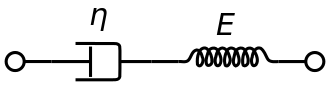
\includegraphics{images/maxwell.png} We can see that following a
deformation, the damper element will not return to it's initial length,
and therre is therefore an element of permanent deformation. We can
therefore discount this model, as it clearly does not represent the
situation wee are trying to model, that of a boxing glove.

    \subsubsection{Kelvin-Voigt Model}\label{kelvin-voigt-model}

The Kelvin-Voigt model is described by a damper and spring mounted in
parallel to one another, as seen in the diagram below.
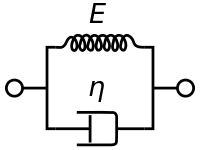
\includegraphics{images/kelvin-voigt.png} We can see that unlike the
Maxwell model, when the Kelvin-Voigt system is compressed and released,
it will return to its initial size. This is representative of the system
we are seeking to model, and can therefore be explored further.

    \subsubsection{Standard Linear Solid
Model}\label{standard-linear-solid-model}

The standard linear solid model (SLSM) can be represented in one of two
ways, however both of these ways overcome the inability of the basic
Maxwell model to return to its initial size when unloaded. We will
consider both models below. \#\#\#\# Maxwell representation of the SLSM
The maxwell representation of the standard linear solid model is
described as a spring in parallel with a basic Maxwell model (i.e. a
spring and damper in series) as described in the diagram below.
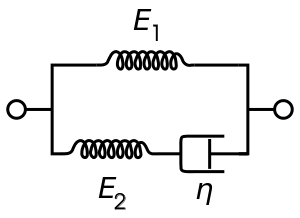
\includegraphics{images/standard-maxwell.png}

\paragraph{Kelvin-Voigt representation of the
SLSM}\label{kelvin-voigt-representation-of-the-slsm}

The Kelvin-Voigt representation of the standard linear solid model is
described as a spring in series with a basic Kelvin-Voigt model (i.e. a
spring and damper in parallel), as described in the diagram below.
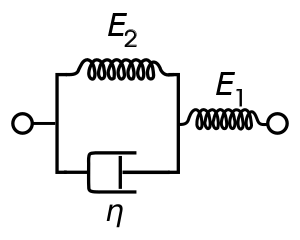
\includegraphics{images/standard-kelvin-voigt.png}

We will therefore consider the latter three models, ignoring only the
basic maxwell model.

    \subsection{Part 2: Equations behind the
Models}\label{part-2-equations-behind-the-models}

We will now seek to write the
equations for each of these three models. We will write out the
differential equations in full, and we will write them iteratively for a
given time step up to a first order approximation, in order to implement
them programatically. We will write as $k_i$ the spring constants, and
$\eta_i$ the dmaping constants, with $\sigma = \frac{F}{A}$ the
stress, and $\eps = \frac{\Delta L}{L}$ the strain, where $F$ is the
force, $A$ the surface area, and $L$ the length. \#\#\# Kelvin-Voigt

Differential Equation: $\sigma = k\eps + \eta \dot{\eps}$

Iterative equation:
$\sigma_{t+\delta t} = k \eps_t + \eta \dot{\eps}_t$

\subsubsection{Maxwell representation of the standard linear solid
model}\label{maxwell-representation-of-the-standard-linear-solid-model}

Differential Equation:
$\sigma + \frac{\eta}{k_2}\dot{\sigma} = k_1\eps + \frac{\eta(k_1 + k_2)}{k_2}\dot{\eps}$

Iterative equation:
$\sigma_{t+\delta t} = k_1\eps_t + \frac{\eta(k_1 + k_2)}{k_2}\dot{\eps}_t - \frac{\eta}{k_2}\dot{\sigma}_t$

$\dot{\sigma}_{t+\delta t} = \frac{k_2}{\eta}\left(k_1\eps_t + \frac{\eta(k_1 + k_2)}{k_2}\dot{\eps}_t - \sigma_t \right)$

\subsubsection{Kelvin-Voigt representation of the standard linear solid
model}\label{kelvin-voigt-representation-of-the-standard-linear-solid-model}

Differential Equation:
$\sigma + \frac{\eta}{k_1+k_2}\dot{\sigma} = \frac{k_1k_2}{K-1+k_2}\eps + \frac{k_1\eta}{k_1+k2}\dot{\eps}$

Iterative equation:
$\sigma_{t+\delta t} = \frac{k_1k_2}{k_1+k_2}\eps_t + \frac{k_1\eta_t}{k_1+k_2}\dot{\eps}_t - \frac{\eta}{k_1+k_2}\dot{\sigma}_t$

$\dot{\sigma}_{t+\delta t} = \frac{k_1+k_2}{\eta}\left(\frac{k_1k_2}{k_1+k_2}\eps_t + \frac{k_1\eta_t}{k_1+k_2}\dot{\eps}_t - \sigma_t \right)$

\paragraph{General remarks on iterative
modelling}\label{general-remarks-on-iterative-modelling}

For all three cases, when treating the model iteratively, we will have

$\eps_{t+\delta t} = \eps_t + \delta t \dot{\eps}_t$

$\dot{\eps}_{t+\delta t} = \dot{\eps}_{t} + \delta t \ddot{\eps}_t$

$\ddot{\eps}_{t+\delta t} = \frac{A}{m}\sigma_{t+\delta t}$

    \subsection{Part 3: Implementing the models - Impact
case:}\label{part-3-implementing-the-models---impact-case}

We are interested in the behaviour of the model immediately after an
impact. We will consider the basic case of a visco-eelastic solid
impacting a rigid surface with a velocity $v_0$ downwards, and driven
by a force $F_0$. We therefore initialise $\dot{\eps}(t=0) = v_0$,
and all other parameters are initialised to 0. The value used for
$F_0$ is characteristic for a punch, which is around
$80g \approx 800 \, N$

    \begin{Verbatim}[commandchars=\\\{\}]
{\color{incolor}In [{\color{incolor}30}]:} \PY{c+c1}{\PYZsh{}\PYZsh{}\PYZsh{} Import Necessary packages}
         \PY{k+kn}{import} \PY{n+nn}{numpy} \PY{k}{as} \PY{n+nn}{np}
         \PY{o}{\PYZpc{}}\PY{k}{matplotlib} notebook
         \PY{k+kn}{import} \PY{n+nn}{matplotlib}\PY{n+nn}{.}\PY{n+nn}{pyplot} \PY{k}{as} \PY{n+nn}{plt}
         
         \PY{c+c1}{\PYZsh{}\PYZsh{}\PYZsh{} Initialise model parameters:}
         \PY{n}{m} \PY{o}{=} \PY{l+m+mf}{0.4} \PY{c+c1}{\PYZsh{} mass (approx. mass of a boxing glove)}
         \PY{n}{k} \PY{o}{=} \PY{l+m+mi}{22000} \PY{c+c1}{\PYZsh{} Single\PYZhy{}spring constant (approx. for rubber foam)}
         \PY{n}{eta} \PY{o}{=} \PY{l+m+mi}{800}\PY{c+c1}{\PYZsh{} single\PYZhy{}damper constant}
         \PY{n}{A} \PY{o}{=} \PY{l+m+mf}{0.01} \PY{c+c1}{\PYZsh{} Surface}
         \PY{n}{F\PYZus{}0} \PY{o}{=} \PY{l+m+mi}{800} \PY{c+c1}{\PYZsh{} Constant force applied}
         
         \PY{c+c1}{\PYZsh{}\PYZsh{}\PYZsh{} Variable Initialisation}
         \PY{n}{e} \PY{o}{=} \PY{l+m+mi}{0} \PY{c+c1}{\PYZsh{} Initial strain}
         \PY{n}{ev} \PY{o}{=} \PY{l+m+mi}{1} \PY{c+c1}{\PYZsh{} Initial strain speed}
         \PY{n}{ea} \PY{o}{=} \PY{l+m+mi}{0} \PY{c+c1}{\PYZsh{} Initial strain acceleration}
         \PY{n}{sig} \PY{o}{=} \PY{l+m+mi}{0} \PY{c+c1}{\PYZsh{} Initial stress}
         \PY{n}{sigv} \PY{o}{=} \PY{n}{ev}\PY{o}{*}\PY{n}{eta} \PY{c+c1}{\PYZsh{} Initial stress speed}
\end{Verbatim}


    \subsubsection{Kelvin-Voigt}\label{kelvin-voigt}

\begin{figure}
\centering
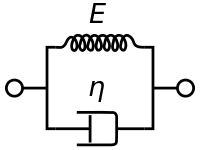
\includegraphics{images/kelvin-voigt.png}
\caption{title}
\end{figure}

$\sigma_{t+\delta t} = k \eps_t + \eta \dot{\eps}_t$

    \begin{Verbatim}[commandchars=\\\{\}]
{\color{incolor}In [{\color{incolor}31}]:} \PY{k}{def} \PY{n+nf}{kelvin\PYZus{}voigt\PYZus{}iter}\PY{p}{(}\PY{n}{e}\PY{p}{,}\PY{n}{ev}\PY{p}{,}\PY{n}{ea}\PY{p}{,}\PY{n}{sig}\PY{p}{,}\PY{n}{dt}\PY{p}{)}\PY{p}{:}
             \PY{c+c1}{\PYZsh{} Define iterative function for definining t+dt from point t according to kelvin\PYZhy{}voigt model.}
             \PY{n}{signew} \PY{o}{=} \PY{p}{(}\PY{n}{k}\PY{o}{*}\PY{n}{e} \PY{o}{+} \PY{n}{eta}\PY{o}{*}\PY{n}{ev}\PY{p}{)} \PY{k}{if} \PY{n}{e}\PY{o}{\PYZgt{}}\PY{o}{=}\PY{l+m+mi}{0} \PY{k}{else} \PY{l+m+mi}{0} \PY{c+c1}{\PYZsh{} define force at t+dt from constitutive equation}
             \PY{n}{eanew} \PY{o}{=} \PY{p}{(}\PY{n}{A}\PY{o}{/}\PY{n}{m}\PY{p}{)}\PY{o}{*}\PY{p}{(}\PY{n}{F\PYZus{}0} \PY{o}{\PYZhy{}} \PY{n}{signew}\PY{p}{)} \PY{c+c1}{\PYZsh{} Define acceleration from force}
             \PY{n}{evnew} \PY{o}{=} \PY{n}{ev} \PY{o}{+} \PY{n}{dt}\PY{o}{*}\PY{n}{eanew} \PY{c+c1}{\PYZsh{} Define velocity from old velocity and acceleration}
             \PY{n}{enew} \PY{o}{=} \PY{n}{e} \PY{o}{+} \PY{n}{dt}\PY{o}{*}\PY{n}{evnew} \PY{c+c1}{\PYZsh{}Define strain from old strain and velocity}
             \PY{k}{return} \PY{n}{enew}\PY{p}{,} \PY{n}{evnew}\PY{p}{,} \PY{n}{eanew}\PY{p}{,} \PY{n}{signew}
             
\end{Verbatim}


    \begin{Verbatim}[commandchars=\\\{\}]
{\color{incolor}In [{\color{incolor}32}]:} \PY{k}{def} \PY{n+nf}{kelvin\PYZus{}voigt}\PY{p}{(}\PY{n}{e\PYZus{}init}\PY{p}{,}\PY{n}{ev\PYZus{}init}\PY{p}{,}\PY{n}{ea\PYZus{}init}\PY{p}{,}\PY{n}{sig\PYZus{}init}\PY{p}{,}\PY{n}{dt}\PY{p}{,}\PY{n}{N}\PY{p}{)}\PY{p}{:}
             \PY{c+c1}{\PYZsh{}Defines the full loop of kelvin voigt model, performing iteeratve step N times, with step dt.}
             \PY{p}{(}\PY{n}{e}\PY{p}{,}\PY{n}{ev}\PY{p}{,}\PY{n}{ea}\PY{p}{,}\PY{n}{sig}\PY{p}{)} \PY{o}{=} \PY{p}{(}\PY{n}{e\PYZus{}init}\PY{p}{,}\PY{n}{ev\PYZus{}init}\PY{p}{,}\PY{n}{ea\PYZus{}init}\PY{p}{,}\PY{n}{sig\PYZus{}init}\PY{p}{)}
             \PY{p}{(}\PY{n}{elist}\PY{p}{,}\PY{n}{evlist}\PY{p}{,}\PY{n}{ealist}\PY{p}{,}\PY{n}{siglist}\PY{p}{)} \PY{o}{=} \PY{p}{(}\PY{p}{[}\PY{n}{e}\PY{p}{]}\PY{p}{,}\PY{p}{[}\PY{n}{ev}\PY{p}{]}\PY{p}{,}\PY{p}{[}\PY{n}{ea}\PY{p}{]}\PY{p}{,}\PY{p}{[}\PY{n}{sig}\PY{p}{]}\PY{p}{)}
             \PY{k}{for} \PY{n}{i} \PY{o+ow}{in} \PY{n+nb}{range}\PY{p}{(}\PY{n}{N}\PY{p}{)}\PY{p}{:}
                 \PY{p}{(}\PY{n}{enew}\PY{p}{,}\PY{n}{evnew}\PY{p}{,}\PY{n}{eanew}\PY{p}{,}\PY{n}{signew}\PY{p}{)} \PY{o}{=} \PY{n}{kelvin\PYZus{}voigt\PYZus{}iter}\PY{p}{(}\PY{n}{e}\PY{p}{,}\PY{n}{ev}\PY{p}{,}\PY{n}{ea}\PY{p}{,}\PY{n}{sig}\PY{p}{,}\PY{n}{dt}\PY{p}{)}
                 \PY{n}{elist}\PY{o}{.}\PY{n}{append}\PY{p}{(}\PY{n}{enew}\PY{p}{)}
                 \PY{n}{evlist}\PY{o}{.}\PY{n}{append}\PY{p}{(}\PY{n}{evnew}\PY{p}{)}
                 \PY{n}{ealist}\PY{o}{.}\PY{n}{append}\PY{p}{(}\PY{n}{eanew}\PY{p}{)}
                 \PY{n}{siglist}\PY{o}{.}\PY{n}{append}\PY{p}{(}\PY{n}{signew}\PY{p}{)}
                 \PY{p}{(}\PY{n}{e}\PY{p}{,}\PY{n}{ev}\PY{p}{,}\PY{n}{ea}\PY{p}{,}\PY{n}{sig}\PY{p}{)} \PY{o}{=} \PY{p}{(}\PY{n}{enew}\PY{p}{,}\PY{n}{evnew}\PY{p}{,}\PY{n}{eanew}\PY{p}{,}\PY{n}{signew}\PY{p}{)}
             \PY{k}{return} \PY{n}{elist}\PY{p}{,}\PY{n}{evlist}\PY{p}{,}\PY{n}{ealist}\PY{p}{,}\PY{n}{siglist}
\end{Verbatim}


    \begin{Verbatim}[commandchars=\\\{\}]
{\color{incolor}In [{\color{incolor}33}]:} \PY{p}{(}\PY{n}{el}\PY{p}{,}\PY{n}{evl}\PY{p}{,}\PY{n}{eal}\PY{p}{,}\PY{n}{sigl}\PY{p}{)} \PY{o}{=} \PY{n}{kelvin\PYZus{}voigt}\PY{p}{(}\PY{n}{e}\PY{p}{,}\PY{n}{ev}\PY{p}{,}\PY{n}{ea}\PY{p}{,}\PY{n}{sig}\PY{p}{,}\PY{l+m+mf}{0.001}\PY{p}{,}\PY{l+m+mi}{2000}\PY{p}{)}
\end{Verbatim}


    \begin{Verbatim}[commandchars=\\\{\}]
{\color{incolor}In [{\color{incolor}34}]:} \PY{n}{plt}\PY{o}{.}\PY{n}{figure}\PY{p}{(}\PY{n}{figsize}\PY{o}{=}\PY{p}{(}\PY{l+m+mi}{9}\PY{p}{,}\PY{l+m+mi}{6}\PY{p}{)}\PY{p}{)}
         \PY{n}{plt}\PY{o}{.}\PY{n}{xlabel}\PY{p}{(}\PY{l+s+s1}{\PYZsq{}}\PY{l+s+s1}{Time}\PY{l+s+s1}{\PYZsq{}}\PY{p}{)}
         \PY{n}{plt}\PY{o}{.}\PY{n}{subplot}\PY{p}{(}\PY{l+m+mi}{221}\PY{p}{)}
         \PY{n}{plt}\PY{o}{.}\PY{n}{title}\PY{p}{(}\PY{l+s+s1}{\PYZsq{}}\PY{l+s+s1}{stress}\PY{l+s+s1}{\PYZsq{}}\PY{p}{)}
         \PY{n}{plt}\PY{o}{.}\PY{n}{plot}\PY{p}{(}\PY{n}{sigl}\PY{p}{)}
         \PY{n}{plt}\PY{o}{.}\PY{n}{subplot}\PY{p}{(}\PY{l+m+mi}{222}\PY{p}{)}
         \PY{n}{plt}\PY{o}{.}\PY{n}{title}\PY{p}{(}\PY{l+s+s1}{\PYZsq{}}\PY{l+s+s1}{strain}\PY{l+s+s1}{\PYZsq{}}\PY{p}{)}
         \PY{n}{plt}\PY{o}{.}\PY{n}{plot}\PY{p}{(}\PY{n}{el}\PY{p}{)}
         \PY{n}{plt}\PY{o}{.}\PY{n}{subplot}\PY{p}{(}\PY{l+m+mi}{223}\PY{p}{)}
         \PY{n}{plt}\PY{o}{.}\PY{n}{title}\PY{p}{(}\PY{l+s+s1}{\PYZsq{}}\PY{l+s+s1}{speed}\PY{l+s+s1}{\PYZsq{}}\PY{p}{)}
         \PY{n}{plt}\PY{o}{.}\PY{n}{plot}\PY{p}{(}\PY{n}{evl}\PY{p}{)}
         \PY{n}{plt}\PY{o}{.}\PY{n}{show}\PY{p}{(}\PY{p}{)}
\end{Verbatim}


    
    \begin{verbatim}
<IPython.core.display.Javascript object>
    \end{verbatim}

    
    
    \begin{verbatim}
<IPython.core.display.HTML object>
    \end{verbatim}

    
    \subsubsection{Standard Linear Solid Model - Maxwell
Representation}\label{standard-linear-solid-model---maxwell-representation}

\begin{figure}
\centering
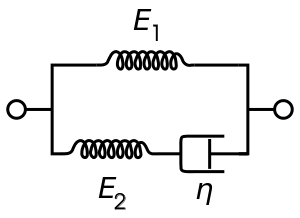
\includegraphics{images/standard-maxwell.png}
\caption{title}
\end{figure}

$\sigma_{t+\delta t} = k_1\eps_t + \frac{\eta(k_1 + k_2)}{k_2}\dot{\eps}_t - \frac{\eta}{k_2}\dot{\sigma}_t$

$\dot{\sigma}_{t+\delta t} = \frac{k_2}{\eta}\left(k_1\eps_t + \frac{\eta(k_1 + k_2)}{k_2}\dot{\eps}_t - \sigma_t \right)$

    \begin{Verbatim}[commandchars=\\\{\}]
{\color{incolor}In [{\color{incolor}35}]:} \PY{c+c1}{\PYZsh{}\PYZsh{}\PYZsh{} Initialise Parameters}
         \PY{n}{k1} \PY{o}{=} \PY{l+m+mi}{12000} \PY{c+c1}{\PYZsh{} Double\PYZhy{}spring constant 1}
         \PY{n}{k2} \PY{o}{=} \PY{l+m+mi}{20000} \PY{c+c1}{\PYZsh{} Double\PYZhy{}spring constant 2}
         \PY{n}{eta} \PY{o}{=} \PY{l+m+mi}{800} \PY{c+c1}{\PYZsh{} Damping constant}
\end{Verbatim}


    \begin{Verbatim}[commandchars=\\\{\}]
{\color{incolor}In [{\color{incolor}36}]:} \PY{k}{def} \PY{n+nf}{SLSM\PYZus{}maxwell\PYZus{}iter}\PY{p}{(}\PY{n}{e}\PY{p}{,}\PY{n}{ev}\PY{p}{,}\PY{n}{ea}\PY{p}{,}\PY{n}{sig}\PY{p}{,}\PY{n}{sigv}\PY{p}{,}\PY{n}{dt}\PY{p}{)}\PY{p}{:}
             \PY{c+c1}{\PYZsh{} Define iterative function for definining t+dt from point t according to SLSM\PYZhy{}Maxwell model.}
             \PY{n}{sigvnew} \PY{o}{=} \PY{p}{(}\PY{n}{k2}\PY{o}{/}\PY{n}{eta}\PY{p}{)}\PY{o}{*}\PY{p}{(}\PY{n}{k1}\PY{o}{*}\PY{n}{e} \PY{o}{+} \PY{n}{ev}\PY{o}{*}\PY{p}{(}\PY{n}{eta}\PY{o}{*}\PY{p}{(}\PY{n}{k1}\PY{o}{+}\PY{n}{k2}\PY{p}{)}\PY{p}{)}\PY{o}{/}\PY{n}{k2} \PY{o}{\PYZhy{}} \PY{n}{sig}\PY{p}{)} \PY{k}{if} \PY{n}{e}\PY{o}{\PYZgt{}}\PY{o}{=}\PY{l+m+mi}{0} \PY{k}{else} \PY{l+m+mi}{0} \PY{c+c1}{\PYZsh{} define force speed at t+dt from constitutive equation}
             \PY{n}{signew} \PY{o}{=}  \PY{n}{sig} \PY{o}{+} \PY{n}{dt}\PY{o}{*}\PY{n}{sigvnew} \PY{k}{if} \PY{n}{e}\PY{o}{\PYZgt{}}\PY{o}{=}\PY{l+m+mi}{0} \PY{k}{else} \PY{l+m+mi}{0} \PY{c+c1}{\PYZsh{} define force at t+dt from constitutive equation k1*e + ev*(eta*(k1+k2))/k2 \PYZhy{} (eta/k2)*sigv}
             \PY{n}{eanew} \PY{o}{=} \PY{p}{(}\PY{n}{A}\PY{o}{/}\PY{n}{m}\PY{p}{)}\PY{o}{*}\PY{p}{(}\PY{n}{F\PYZus{}0} \PY{o}{\PYZhy{}} \PY{n}{signew}\PY{p}{)} \PY{c+c1}{\PYZsh{} Define acceleration from force}
             \PY{n}{evnew} \PY{o}{=} \PY{n}{ev} \PY{o}{+} \PY{n}{dt}\PY{o}{*}\PY{n}{eanew} \PY{c+c1}{\PYZsh{} Define velocity from old velocity and acceleration}
             \PY{n}{enew} \PY{o}{=} \PY{n}{e} \PY{o}{+} \PY{n}{dt}\PY{o}{*}\PY{n}{evnew} \PY{c+c1}{\PYZsh{}Define strain from old strain and velocity}
             \PY{k}{return} \PY{n}{enew}\PY{p}{,} \PY{n}{evnew}\PY{p}{,} \PY{n}{eanew}\PY{p}{,} \PY{n}{signew}\PY{p}{,} \PY{n}{sigvnew}
             
\end{Verbatim}


    \begin{Verbatim}[commandchars=\\\{\}]
{\color{incolor}In [{\color{incolor}37}]:} \PY{k}{def} \PY{n+nf}{SLSM\PYZus{}maxwell}\PY{p}{(}\PY{n}{e\PYZus{}init}\PY{p}{,}\PY{n}{ev\PYZus{}init}\PY{p}{,}\PY{n}{ea\PYZus{}init}\PY{p}{,}\PY{n}{sig\PYZus{}init}\PY{p}{,}\PY{n}{sigv\PYZus{}init}\PY{p}{,}\PY{n}{dt}\PY{p}{,}\PY{n}{N}\PY{p}{)}\PY{p}{:}
             \PY{c+c1}{\PYZsh{}Defines the full loop of SLSM\PYZhy{}maxwell model, performing iteeratve step N times, with step dt.}
             \PY{p}{(}\PY{n}{e}\PY{p}{,}\PY{n}{ev}\PY{p}{,}\PY{n}{ea}\PY{p}{,}\PY{n}{sig}\PY{p}{,}\PY{n}{sigv}\PY{p}{)} \PY{o}{=} \PY{p}{(}\PY{n}{e\PYZus{}init}\PY{p}{,}\PY{n}{ev\PYZus{}init}\PY{p}{,}\PY{n}{ea\PYZus{}init}\PY{p}{,}\PY{n}{sig\PYZus{}init}\PY{p}{,}\PY{n}{sigv\PYZus{}init}\PY{p}{)}
             \PY{p}{(}\PY{n}{elist}\PY{p}{,}\PY{n}{evlist}\PY{p}{,}\PY{n}{ealist}\PY{p}{,}\PY{n}{siglist}\PY{p}{,}\PY{n}{sigvlist}\PY{p}{)} \PY{o}{=} \PY{p}{(}\PY{p}{[}\PY{n}{e}\PY{p}{]}\PY{p}{,}\PY{p}{[}\PY{n}{ev}\PY{p}{]}\PY{p}{,}\PY{p}{[}\PY{n}{ea}\PY{p}{]}\PY{p}{,}\PY{p}{[}\PY{n}{sig}\PY{p}{]}\PY{p}{,}\PY{p}{[}\PY{n}{sigv}\PY{p}{]}\PY{p}{)}
             \PY{k}{for} \PY{n}{i} \PY{o+ow}{in} \PY{n+nb}{range}\PY{p}{(}\PY{n}{N}\PY{p}{)}\PY{p}{:}
                 \PY{p}{(}\PY{n}{enew}\PY{p}{,}\PY{n}{evnew}\PY{p}{,}\PY{n}{eanew}\PY{p}{,}\PY{n}{signew}\PY{p}{,}\PY{n}{sigvnew}\PY{p}{)} \PY{o}{=} \PY{n}{SLSM\PYZus{}maxwell\PYZus{}iter}\PY{p}{(}\PY{n}{e}\PY{p}{,}\PY{n}{ev}\PY{p}{,}\PY{n}{ea}\PY{p}{,}\PY{n}{sig}\PY{p}{,}\PY{n}{sigv}\PY{p}{,}\PY{n}{dt}\PY{p}{)}
                 \PY{n}{elist}\PY{o}{.}\PY{n}{append}\PY{p}{(}\PY{n}{enew}\PY{p}{)}
                 \PY{n}{evlist}\PY{o}{.}\PY{n}{append}\PY{p}{(}\PY{n}{evnew}\PY{p}{)}
                 \PY{n}{ealist}\PY{o}{.}\PY{n}{append}\PY{p}{(}\PY{n}{eanew}\PY{p}{)}
                 \PY{n}{siglist}\PY{o}{.}\PY{n}{append}\PY{p}{(}\PY{n}{signew}\PY{p}{)}
                 \PY{n}{sigvlist}\PY{o}{.}\PY{n}{append}\PY{p}{(}\PY{n}{sigvnew}\PY{p}{)}
                 \PY{p}{(}\PY{n}{e}\PY{p}{,}\PY{n}{ev}\PY{p}{,}\PY{n}{ea}\PY{p}{,}\PY{n}{sig}\PY{p}{,}\PY{n}{sigv}\PY{p}{)} \PY{o}{=} \PY{p}{(}\PY{n}{enew}\PY{p}{,}\PY{n}{evnew}\PY{p}{,}\PY{n}{eanew}\PY{p}{,}\PY{n}{signew}\PY{p}{,}\PY{n}{sigvnew}\PY{p}{)}
             \PY{k}{return} \PY{n}{elist}\PY{p}{,}\PY{n}{evlist}\PY{p}{,}\PY{n}{ealist}\PY{p}{,}\PY{n}{siglist}\PY{p}{,}\PY{n}{sigvlist}
\end{Verbatim}


    \begin{Verbatim}[commandchars=\\\{\}]
{\color{incolor}In [{\color{incolor}38}]:} \PY{p}{(}\PY{n}{el}\PY{p}{,}\PY{n}{evl}\PY{p}{,}\PY{n}{eal}\PY{p}{,}\PY{n}{sigl}\PY{p}{,}\PY{n}{sigvl}\PY{p}{)} \PY{o}{=} \PY{n}{SLSM\PYZus{}maxwell}\PY{p}{(}\PY{n}{e}\PY{p}{,}\PY{n}{ev}\PY{p}{,}\PY{n}{ea}\PY{p}{,}\PY{n}{sig}\PY{p}{,}\PY{n}{sigv}\PY{p}{,}\PY{l+m+mf}{0.001}\PY{p}{,}\PY{l+m+mi}{2000}\PY{p}{)}
\end{Verbatim}


    \begin{Verbatim}[commandchars=\\\{\}]
{\color{incolor}In [{\color{incolor}39}]:} \PY{n}{plt}\PY{o}{.}\PY{n}{figure}\PY{p}{(}\PY{n}{figsize}\PY{o}{=}\PY{p}{(}\PY{l+m+mi}{9}\PY{p}{,}\PY{l+m+mi}{6}\PY{p}{)}\PY{p}{)}
         \PY{n}{plt}\PY{o}{.}\PY{n}{xlabel}\PY{p}{(}\PY{l+s+s1}{\PYZsq{}}\PY{l+s+s1}{Time}\PY{l+s+s1}{\PYZsq{}}\PY{p}{)}
         \PY{n}{plt}\PY{o}{.}\PY{n}{subplot}\PY{p}{(}\PY{l+m+mi}{221}\PY{p}{)}
         \PY{n}{plt}\PY{o}{.}\PY{n}{title}\PY{p}{(}\PY{l+s+s1}{\PYZsq{}}\PY{l+s+s1}{stress}\PY{l+s+s1}{\PYZsq{}}\PY{p}{)}
         \PY{n}{plt}\PY{o}{.}\PY{n}{plot}\PY{p}{(}\PY{n}{sigl}\PY{p}{)}
         \PY{n}{plt}\PY{o}{.}\PY{n}{subplot}\PY{p}{(}\PY{l+m+mi}{222}\PY{p}{)}
         \PY{n}{plt}\PY{o}{.}\PY{n}{title}\PY{p}{(}\PY{l+s+s1}{\PYZsq{}}\PY{l+s+s1}{strain}\PY{l+s+s1}{\PYZsq{}}\PY{p}{)}
         \PY{n}{plt}\PY{o}{.}\PY{n}{plot}\PY{p}{(}\PY{n}{el}\PY{p}{)}
         \PY{n}{plt}\PY{o}{.}\PY{n}{subplot}\PY{p}{(}\PY{l+m+mi}{223}\PY{p}{)}
         \PY{n}{plt}\PY{o}{.}\PY{n}{title}\PY{p}{(}\PY{l+s+s1}{\PYZsq{}}\PY{l+s+s1}{speed}\PY{l+s+s1}{\PYZsq{}}\PY{p}{)}
         \PY{n}{plt}\PY{o}{.}\PY{n}{plot}\PY{p}{(}\PY{n}{evl}\PY{p}{)}
         \PY{n}{plt}\PY{o}{.}\PY{n}{subplot}\PY{p}{(}\PY{l+m+mi}{224}\PY{p}{)}
         \PY{n}{plt}\PY{o}{.}\PY{n}{title}\PY{p}{(}\PY{l+s+s1}{\PYZsq{}}\PY{l+s+s1}{stress speed}\PY{l+s+s1}{\PYZsq{}}\PY{p}{)}
         \PY{n}{plt}\PY{o}{.}\PY{n}{plot}\PY{p}{(}\PY{n}{sigvl}\PY{p}{)}
         \PY{n}{plt}\PY{o}{.}\PY{n}{show}\PY{p}{(}\PY{p}{)}
\end{Verbatim}


    
    \begin{verbatim}
<IPython.core.display.Javascript object>
    \end{verbatim}

    
    
    \begin{verbatim}
<IPython.core.display.HTML object>
    \end{verbatim}

    
    \subsubsection{Standard Linear Solid Model - Kelvin-Voigt
Representation}\label{standard-linear-solid-model---kelvin-voigt-representation}

\begin{figure}
\centering
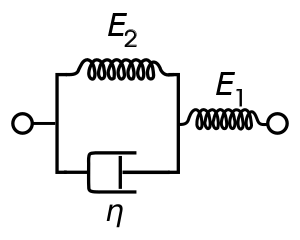
\includegraphics{images/standard-kelvin-voigt.png}
\caption{title}
\end{figure}

$\sigma_{t+\delta t} = \frac{k_1k_2}{k_1+k_2}\eps_t + \frac{k_1\eta_t}{k_1+k_2}\dot{\eps}_t - \frac{\eta}{k_1+k_2}\dot{\sigma}_t$

$\dot{\sigma}_{t+\delta t} = \frac{k_1+k_2}{\eta}\left(\frac{k_1k_2}{k_1+k_2}\eps_t + \frac{k_1\eta_t}{k_1+k_2}\dot{\eps}_t - \sigma_t \right)$

    \begin{Verbatim}[commandchars=\\\{\}]
{\color{incolor}In [{\color{incolor}40}]:} \PY{c+c1}{\PYZsh{}\PYZsh{}\PYZsh{} Initialise Parameters}
         \PY{n}{k1} \PY{o}{=} \PY{l+m+mi}{60000} \PY{c+c1}{\PYZsh{} Double\PYZhy{}spring constant 1}
         \PY{n}{k2} \PY{o}{=} \PY{l+m+mi}{30000} \PY{c+c1}{\PYZsh{} Double\PYZhy{}spring constant 2}
         \PY{n}{eta} \PY{o}{=} \PY{l+m+mi}{1000} \PY{c+c1}{\PYZsh{} Damping constant}
         \PY{n}{sig} \PY{o}{=} \PY{l+m+mi}{0} \PY{c+c1}{\PYZsh{}e*k1*k2/(k1+k2) + ev*(eta*k1)/(k1+k2)}
\end{Verbatim}


    \begin{Verbatim}[commandchars=\\\{\}]
{\color{incolor}In [{\color{incolor}41}]:} \PY{k}{def} \PY{n+nf}{SLSM\PYZus{}kelvin\PYZus{}voigt\PYZus{}iter}\PY{p}{(}\PY{n}{e}\PY{p}{,}\PY{n}{ev}\PY{p}{,}\PY{n}{ea}\PY{p}{,}\PY{n}{sig}\PY{p}{,}\PY{n}{sigv}\PY{p}{,}\PY{n}{dt}\PY{p}{)}\PY{p}{:}
             \PY{c+c1}{\PYZsh{} Define iterative function for definining t+dt from point t according to SLSM\PYZhy{}kelvin\PYZhy{}voigt model.}
             \PY{n}{sigvnew} \PY{o}{=} \PY{p}{(}\PY{n}{k1}\PY{o}{+}\PY{n}{k2}\PY{o}{/}\PY{n}{eta}\PY{p}{)}\PY{o}{*}\PY{p}{(}\PY{n}{e}\PY{o}{*}\PY{n}{k1}\PY{o}{*}\PY{n}{k2}\PY{o}{/}\PY{p}{(}\PY{n}{k1}\PY{o}{+}\PY{n}{k2}\PY{p}{)} \PY{o}{+} \PY{n}{ev}\PY{o}{*}\PY{p}{(}\PY{n}{eta}\PY{o}{*}\PY{n}{k1}\PY{p}{)}\PY{o}{/}\PY{p}{(}\PY{n}{k1}\PY{o}{+}\PY{n}{k2}\PY{p}{)} \PY{o}{\PYZhy{}} \PY{n}{sig}\PY{p}{)} \PY{k}{if} \PY{n}{e}\PY{o}{\PYZgt{}}\PY{o}{=}\PY{l+m+mi}{0} \PY{k}{else} \PY{l+m+mi}{0} \PY{c+c1}{\PYZsh{} define force speed at t+dt from constitutive equation}
             \PY{n}{signew} \PY{o}{=}  \PY{n}{sig} \PY{o}{+} \PY{n}{dt}\PY{o}{*}\PY{n}{sigvnew} \PY{k}{if} \PY{n}{e}\PY{o}{\PYZgt{}}\PY{o}{=}\PY{l+m+mi}{0} \PY{k}{else} \PY{l+m+mi}{0} \PY{c+c1}{\PYZsh{} define force at t+dt from constitutive equation}
             \PY{c+c1}{\PYZsh{} signew = e*k1*k2/(k1+k2) + ev*k1*eta/(k1+k2) \PYZhy{}  eta*sigv/(k1+k2) if e\PYZgt{}=0 else 0}
             \PY{c+c1}{\PYZsh{} sigvnew = (k1+k2/eta)*(e*k1*k2/(k1+k2) + ev*(eta*k1)/(k1+k2) \PYZhy{} sig)}
             \PY{n}{eanew} \PY{o}{=} \PY{p}{(}\PY{n}{A}\PY{o}{/}\PY{n}{m}\PY{p}{)}\PY{o}{*}\PY{p}{(}\PY{n}{F\PYZus{}0} \PY{o}{\PYZhy{}} \PY{n}{signew}\PY{p}{)} \PY{c+c1}{\PYZsh{} Define acceleration from force}
             \PY{n}{evnew} \PY{o}{=} \PY{n}{ev} \PY{o}{+} \PY{n}{dt}\PY{o}{*}\PY{n}{eanew} \PY{c+c1}{\PYZsh{} Define velocity from old velocity and acceleration}
             \PY{n}{enew} \PY{o}{=} \PY{n}{e} \PY{o}{+} \PY{n}{dt}\PY{o}{*}\PY{n}{evnew} \PY{c+c1}{\PYZsh{}Define strain from old strain and velocity}
             \PY{k}{return} \PY{n}{enew}\PY{p}{,} \PY{n}{evnew}\PY{p}{,} \PY{n}{eanew}\PY{p}{,} \PY{n}{signew}\PY{p}{,} \PY{n}{sigvnew}
\end{Verbatim}


    \begin{Verbatim}[commandchars=\\\{\}]
{\color{incolor}In [{\color{incolor}42}]:} \PY{k}{def} \PY{n+nf}{SLSM\PYZus{}kelvin\PYZus{}voigt}\PY{p}{(}\PY{n}{e\PYZus{}init}\PY{p}{,}\PY{n}{ev\PYZus{}init}\PY{p}{,}\PY{n}{ea\PYZus{}init}\PY{p}{,}\PY{n}{sig\PYZus{}init}\PY{p}{,}\PY{n}{sigv\PYZus{}init}\PY{p}{,}\PY{n}{dt}\PY{p}{,}\PY{n}{N}\PY{p}{)}\PY{p}{:}
             \PY{c+c1}{\PYZsh{}Defines the full loop of SLSM\PYZhy{}kelvin\PYZhy{}voigt model, performing iteratve step N times, with step dt.}
             \PY{p}{(}\PY{n}{e}\PY{p}{,}\PY{n}{ev}\PY{p}{,}\PY{n}{ea}\PY{p}{,}\PY{n}{sig}\PY{p}{,}\PY{n}{sigv}\PY{p}{)} \PY{o}{=} \PY{p}{(}\PY{n}{e\PYZus{}init}\PY{p}{,}\PY{n}{ev\PYZus{}init}\PY{p}{,}\PY{n}{ea\PYZus{}init}\PY{p}{,}\PY{n}{sig\PYZus{}init}\PY{p}{,}\PY{n}{sigv\PYZus{}init}\PY{p}{)}
             \PY{p}{(}\PY{n}{elist}\PY{p}{,}\PY{n}{evlist}\PY{p}{,}\PY{n}{ealist}\PY{p}{,}\PY{n}{siglist}\PY{p}{,}\PY{n}{sigvlist}\PY{p}{)} \PY{o}{=} \PY{p}{(}\PY{p}{[}\PY{n}{e}\PY{p}{]}\PY{p}{,}\PY{p}{[}\PY{n}{ev}\PY{p}{]}\PY{p}{,}\PY{p}{[}\PY{n}{ea}\PY{p}{]}\PY{p}{,}\PY{p}{[}\PY{n}{sig}\PY{p}{]}\PY{p}{,}\PY{p}{[}\PY{n}{sigv}\PY{p}{]}\PY{p}{)}
             \PY{k}{for} \PY{n}{i} \PY{o+ow}{in} \PY{n+nb}{range}\PY{p}{(}\PY{n}{N}\PY{p}{)}\PY{p}{:}
                 \PY{p}{(}\PY{n}{enew}\PY{p}{,}\PY{n}{evnew}\PY{p}{,}\PY{n}{eanew}\PY{p}{,}\PY{n}{signew}\PY{p}{,}\PY{n}{sigvnew}\PY{p}{)} \PY{o}{=} \PY{n}{SLSM\PYZus{}kelvin\PYZus{}voigt\PYZus{}iter}\PY{p}{(}\PY{n}{e}\PY{p}{,}\PY{n}{ev}\PY{p}{,}\PY{n}{ea}\PY{p}{,}\PY{n}{sig}\PY{p}{,}\PY{n}{sigv}\PY{p}{,}\PY{n}{dt}\PY{p}{)}
                 \PY{n}{elist}\PY{o}{.}\PY{n}{append}\PY{p}{(}\PY{n}{enew}\PY{p}{)}
                 \PY{n}{evlist}\PY{o}{.}\PY{n}{append}\PY{p}{(}\PY{n}{evnew}\PY{p}{)}
                 \PY{n}{ealist}\PY{o}{.}\PY{n}{append}\PY{p}{(}\PY{n}{eanew}\PY{p}{)}
                 \PY{n}{siglist}\PY{o}{.}\PY{n}{append}\PY{p}{(}\PY{n}{signew}\PY{p}{)}
                 \PY{n}{sigvlist}\PY{o}{.}\PY{n}{append}\PY{p}{(}\PY{n}{sigvnew}\PY{p}{)}
                 \PY{p}{(}\PY{n}{e}\PY{p}{,}\PY{n}{ev}\PY{p}{,}\PY{n}{ea}\PY{p}{,}\PY{n}{sig}\PY{p}{,}\PY{n}{sigv}\PY{p}{)} \PY{o}{=} \PY{p}{(}\PY{n}{enew}\PY{p}{,}\PY{n}{evnew}\PY{p}{,}\PY{n}{eanew}\PY{p}{,}\PY{n}{signew}\PY{p}{,}\PY{n}{sigvnew}\PY{p}{)}
             \PY{k}{return} \PY{n}{elist}\PY{p}{,}\PY{n}{evlist}\PY{p}{,}\PY{n}{ealist}\PY{p}{,}\PY{n}{siglist}\PY{p}{,}\PY{n}{sigvlist}
\end{Verbatim}


    \begin{Verbatim}[commandchars=\\\{\}]
{\color{incolor}In [{\color{incolor}43}]:} \PY{p}{(}\PY{n}{el}\PY{p}{,}\PY{n}{evl}\PY{p}{,}\PY{n}{eal}\PY{p}{,}\PY{n}{sigl}\PY{p}{,}\PY{n}{sigvl}\PY{p}{)} \PY{o}{=} \PY{n}{SLSM\PYZus{}kelvin\PYZus{}voigt}\PY{p}{(}\PY{n}{e}\PY{p}{,}\PY{n}{ev}\PY{p}{,}\PY{n}{ea}\PY{p}{,}\PY{n}{sig}\PY{p}{,}\PY{n}{sigv}\PY{p}{,}\PY{l+m+mf}{0.00001}\PY{p}{,}\PY{l+m+mi}{100000}\PY{p}{)}
\end{Verbatim}


    \begin{Verbatim}[commandchars=\\\{\}]
{\color{incolor}In [{\color{incolor}44}]:} \PY{n}{plt}\PY{o}{.}\PY{n}{figure}\PY{p}{(}\PY{n}{figsize}\PY{o}{=}\PY{p}{(}\PY{l+m+mi}{9}\PY{p}{,}\PY{l+m+mi}{6}\PY{p}{)}\PY{p}{)}
         \PY{n}{plt}\PY{o}{.}\PY{n}{xlabel}\PY{p}{(}\PY{l+s+s1}{\PYZsq{}}\PY{l+s+s1}{Time}\PY{l+s+s1}{\PYZsq{}}\PY{p}{)}
         \PY{n}{plt}\PY{o}{.}\PY{n}{subplot}\PY{p}{(}\PY{l+m+mi}{221}\PY{p}{)}
         \PY{n}{plt}\PY{o}{.}\PY{n}{title}\PY{p}{(}\PY{l+s+s1}{\PYZsq{}}\PY{l+s+s1}{stress}\PY{l+s+s1}{\PYZsq{}}\PY{p}{)}
         \PY{n}{plt}\PY{o}{.}\PY{n}{plot}\PY{p}{(}\PY{n}{sigl}\PY{p}{)}
         \PY{n}{plt}\PY{o}{.}\PY{n}{subplot}\PY{p}{(}\PY{l+m+mi}{222}\PY{p}{)}
         \PY{n}{plt}\PY{o}{.}\PY{n}{title}\PY{p}{(}\PY{l+s+s1}{\PYZsq{}}\PY{l+s+s1}{strain}\PY{l+s+s1}{\PYZsq{}}\PY{p}{)}
         \PY{n}{plt}\PY{o}{.}\PY{n}{plot}\PY{p}{(}\PY{n}{el}\PY{p}{)}
         \PY{n}{plt}\PY{o}{.}\PY{n}{subplot}\PY{p}{(}\PY{l+m+mi}{223}\PY{p}{)}
         \PY{n}{plt}\PY{o}{.}\PY{n}{title}\PY{p}{(}\PY{l+s+s1}{\PYZsq{}}\PY{l+s+s1}{speed}\PY{l+s+s1}{\PYZsq{}}\PY{p}{)}
         \PY{n}{plt}\PY{o}{.}\PY{n}{plot}\PY{p}{(}\PY{n}{evl}\PY{p}{)}
         \PY{n}{plt}\PY{o}{.}\PY{n}{subplot}\PY{p}{(}\PY{l+m+mi}{224}\PY{p}{)}
         \PY{n}{plt}\PY{o}{.}\PY{n}{title}\PY{p}{(}\PY{l+s+s1}{\PYZsq{}}\PY{l+s+s1}{stress speed}\PY{l+s+s1}{\PYZsq{}}\PY{p}{)}
         \PY{n}{i}\PY{o}{=}\PY{l+m+mi}{15}
         \PY{n}{sigvl}\PY{p}{[}\PY{l+m+mi}{0}\PY{p}{:}\PY{n}{i}\PY{p}{]}\PY{o}{=}\PY{p}{[}\PY{n}{sigvl}\PY{p}{[}\PY{n}{i}\PY{p}{]}\PY{p}{]}\PY{o}{*}\PY{n}{i}
         \PY{n}{plt}\PY{o}{.}\PY{n}{plot}\PY{p}{(}\PY{n}{sigvl}\PY{p}{)}
         \PY{n}{plt}\PY{o}{.}\PY{n}{show}\PY{p}{(}\PY{p}{)}
\end{Verbatim}


    
    \begin{verbatim}
<IPython.core.display.Javascript object>
    \end{verbatim}

    
    
    \begin{verbatim}
<IPython.core.display.HTML object>
    \end{verbatim}

    
    \subsection{Part 4: Analysing and Comparing the
models}\label{part-4-analysing-and-comparing-the-models}

Due to the fact that we have different input parameters for each model,
it is very difficult to compare them $\textit{ceteris paribus}$,
however, we can consider each of them individually, and understand their
dependence on theeir various inputs.

\subsubsection{Kelvin - Voigt}\label{kelvin---voigt}

We will start from an arbitrary $\textit{reference}$ configuration,
$(k = 22000 \, N/m,\, \eta = 800 \, Ns/m)$, and vary both parameters
independently. Finally, we will also vary the force, to understand how
this affects the early part of the motion.

    \begin{Verbatim}[commandchars=\\\{\}]
{\color{incolor}In [{\color{incolor}45}]:} \PY{c+c1}{\PYZsh{}\PYZsh{} Comparison at constant eta = 800}
         \PY{n}{eta} \PY{o}{=} \PY{l+m+mi}{800}
         \PY{c+c1}{\PYZsh{}\PYZsh{}\PYZsh{} Variable Initialisation}
         \PY{n}{e} \PY{o}{=} \PY{l+m+mi}{0} \PY{c+c1}{\PYZsh{} Initial strain}
         \PY{n}{ev} \PY{o}{=} \PY{l+m+mi}{1} \PY{c+c1}{\PYZsh{} Initial strain speed}
         \PY{n}{ea} \PY{o}{=} \PY{l+m+mi}{0} \PY{c+c1}{\PYZsh{} Initial strain acceleration}
         \PY{n}{sig} \PY{o}{=} \PY{l+m+mi}{0} \PY{c+c1}{\PYZsh{} Initial stress}
         \PY{n}{k} \PY{o}{=} \PY{l+m+mi}{10000}
         \PY{p}{(}\PY{n}{el1}\PY{p}{,}\PY{n}{evl1}\PY{p}{,}\PY{n}{eal1}\PY{p}{,}\PY{n}{sigl1}\PY{p}{)} \PY{o}{=} \PY{n}{kelvin\PYZus{}voigt}\PY{p}{(}\PY{n}{e}\PY{p}{,}\PY{n}{ev}\PY{p}{,}\PY{n}{ea}\PY{p}{,}\PY{n}{sig}\PY{p}{,}\PY{l+m+mf}{0.0001}\PY{p}{,}\PY{l+m+mi}{10000}\PY{p}{)}
         \PY{n}{k} \PY{o}{=} \PY{l+m+mi}{16000}
         \PY{p}{(}\PY{n}{el2}\PY{p}{,}\PY{n}{evl2}\PY{p}{,}\PY{n}{eal2}\PY{p}{,}\PY{n}{sigl2}\PY{p}{)} \PY{o}{=} \PY{n}{kelvin\PYZus{}voigt}\PY{p}{(}\PY{n}{e}\PY{p}{,}\PY{n}{ev}\PY{p}{,}\PY{n}{ea}\PY{p}{,}\PY{n}{sig}\PY{p}{,}\PY{l+m+mf}{0.0001}\PY{p}{,}\PY{l+m+mi}{10000}\PY{p}{)}
         \PY{n}{k} \PY{o}{=} \PY{l+m+mi}{22000}
         \PY{p}{(}\PY{n}{el3}\PY{p}{,}\PY{n}{evl3}\PY{p}{,}\PY{n}{eal3}\PY{p}{,}\PY{n}{sigl3}\PY{p}{)} \PY{o}{=} \PY{n}{kelvin\PYZus{}voigt}\PY{p}{(}\PY{n}{e}\PY{p}{,}\PY{n}{ev}\PY{p}{,}\PY{n}{ea}\PY{p}{,}\PY{n}{sig}\PY{p}{,}\PY{l+m+mf}{0.0001}\PY{p}{,}\PY{l+m+mi}{10000}\PY{p}{)}
         \PY{n}{k} \PY{o}{=} \PY{l+m+mi}{28000}
         \PY{p}{(}\PY{n}{el4}\PY{p}{,}\PY{n}{evl4}\PY{p}{,}\PY{n}{eal4}\PY{p}{,}\PY{n}{sigl4}\PY{p}{)} \PY{o}{=} \PY{n}{kelvin\PYZus{}voigt}\PY{p}{(}\PY{n}{e}\PY{p}{,}\PY{n}{ev}\PY{p}{,}\PY{n}{ea}\PY{p}{,}\PY{n}{sig}\PY{p}{,}\PY{l+m+mf}{0.0001}\PY{p}{,}\PY{l+m+mi}{10000}\PY{p}{)}
         \PY{n}{k} \PY{o}{=} \PY{l+m+mi}{34000}
         \PY{p}{(}\PY{n}{el5}\PY{p}{,}\PY{n}{evl5}\PY{p}{,}\PY{n}{eal5}\PY{p}{,}\PY{n}{sigl5}\PY{p}{)} \PY{o}{=} \PY{n}{kelvin\PYZus{}voigt}\PY{p}{(}\PY{n}{e}\PY{p}{,}\PY{n}{ev}\PY{p}{,}\PY{n}{ea}\PY{p}{,}\PY{n}{sig}\PY{p}{,}\PY{l+m+mf}{0.0001}\PY{p}{,}\PY{l+m+mi}{10000}\PY{p}{)}
\end{Verbatim}


    \begin{Verbatim}[commandchars=\\\{\}]
{\color{incolor}In [{\color{incolor}46}]:} \PY{n}{plt}\PY{o}{.}\PY{n}{figure}\PY{p}{(}\PY{n}{figsize}\PY{o}{=}\PY{p}{(}\PY{l+m+mi}{9}\PY{p}{,}\PY{l+m+mi}{6}\PY{p}{)}\PY{p}{)}
         \PY{n}{plt}\PY{o}{.}\PY{n}{title}\PY{p}{(}\PY{l+s+s1}{\PYZsq{}}\PY{l+s+s1}{stress}\PY{l+s+s1}{\PYZsq{}}\PY{p}{)}
         \PY{n}{plt}\PY{o}{.}\PY{n}{plot}\PY{p}{(}\PY{n}{sigl1} \PY{p}{,} \PY{n}{label} \PY{o}{=} \PY{l+s+s1}{\PYZsq{}}\PY{l+s+s1}{k = 10000}\PY{l+s+s1}{\PYZsq{}}\PY{p}{)}
         \PY{n}{plt}\PY{o}{.}\PY{n}{plot}\PY{p}{(}\PY{n}{sigl2} \PY{p}{,} \PY{n}{label} \PY{o}{=} \PY{l+s+s1}{\PYZsq{}}\PY{l+s+s1}{k = 16000}\PY{l+s+s1}{\PYZsq{}}\PY{p}{)}
         \PY{n}{plt}\PY{o}{.}\PY{n}{plot}\PY{p}{(}\PY{n}{sigl3} \PY{p}{,} \PY{n}{label} \PY{o}{=} \PY{l+s+s1}{\PYZsq{}}\PY{l+s+s1}{k = 22000}\PY{l+s+s1}{\PYZsq{}}\PY{p}{)}
         \PY{n}{plt}\PY{o}{.}\PY{n}{plot}\PY{p}{(}\PY{n}{sigl4} \PY{p}{,} \PY{n}{label} \PY{o}{=} \PY{l+s+s1}{\PYZsq{}}\PY{l+s+s1}{k = 28000}\PY{l+s+s1}{\PYZsq{}}\PY{p}{)}
         \PY{n}{plt}\PY{o}{.}\PY{n}{plot}\PY{p}{(}\PY{n}{sigl5} \PY{p}{,} \PY{n}{label} \PY{o}{=} \PY{l+s+s1}{\PYZsq{}}\PY{l+s+s1}{k = 32000}\PY{l+s+s1}{\PYZsq{}}\PY{p}{)}
         \PY{n}{plt}\PY{o}{.}\PY{n}{xlabel}\PY{p}{(}\PY{l+s+s1}{\PYZsq{}}\PY{l+s+s1}{time}\PY{l+s+s1}{\PYZsq{}}\PY{p}{)}
         \PY{n}{a}\PY{o}{=}\PY{n}{plt}\PY{o}{.}\PY{n}{legend}\PY{p}{(}\PY{p}{)}
\end{Verbatim}


    
    \begin{verbatim}
<IPython.core.display.Javascript object>
    \end{verbatim}

    
    
    \begin{verbatim}
<IPython.core.display.HTML object>
    \end{verbatim}

    
    \paragraph{Analysis}\label{analysis}

We can see that a higher spring constant corresponds to a higher peak
force, a shorter impact time, and more oscillations.

    \begin{Verbatim}[commandchars=\\\{\}]
{\color{incolor}In [{\color{incolor}47}]:} \PY{c+c1}{\PYZsh{}\PYZsh{} Comparison at constant k = 22000}
         \PY{n}{k} \PY{o}{=} \PY{l+m+mi}{22000}
         \PY{c+c1}{\PYZsh{}\PYZsh{}\PYZsh{} Variable Initialisation}
         \PY{n}{e} \PY{o}{=} \PY{l+m+mi}{0} \PY{c+c1}{\PYZsh{} Initial strain}
         \PY{n}{ev} \PY{o}{=} \PY{l+m+mi}{1} \PY{c+c1}{\PYZsh{} Initial strain speed}
         \PY{n}{ea} \PY{o}{=} \PY{l+m+mi}{0} \PY{c+c1}{\PYZsh{} Initial strain acceleration}
         \PY{n}{sig} \PY{o}{=} \PY{l+m+mi}{0} \PY{c+c1}{\PYZsh{} Initial stress}
         \PY{n}{eta} \PY{o}{=}\PY{l+m+mi}{200}
         \PY{p}{(}\PY{n}{el1}\PY{p}{,}\PY{n}{evl1}\PY{p}{,}\PY{n}{eal1}\PY{p}{,}\PY{n}{sigl1}\PY{p}{)} \PY{o}{=} \PY{n}{kelvin\PYZus{}voigt}\PY{p}{(}\PY{n}{e}\PY{p}{,}\PY{n}{ev}\PY{p}{,}\PY{n}{ea}\PY{p}{,}\PY{n}{sig}\PY{p}{,}\PY{l+m+mf}{0.001}\PY{p}{,}\PY{l+m+mi}{1000}\PY{p}{)}
         \PY{n}{eta} \PY{o}{=} \PY{l+m+mi}{400}
         \PY{p}{(}\PY{n}{el2}\PY{p}{,}\PY{n}{evl2}\PY{p}{,}\PY{n}{eal2}\PY{p}{,}\PY{n}{sigl2}\PY{p}{)} \PY{o}{=} \PY{n}{kelvin\PYZus{}voigt}\PY{p}{(}\PY{n}{e}\PY{p}{,}\PY{n}{ev}\PY{p}{,}\PY{n}{ea}\PY{p}{,}\PY{n}{sig}\PY{p}{,}\PY{l+m+mf}{0.001}\PY{p}{,}\PY{l+m+mi}{1000}\PY{p}{)}
         \PY{n}{eta} \PY{o}{=} \PY{l+m+mi}{800}
         \PY{p}{(}\PY{n}{el3}\PY{p}{,}\PY{n}{evl3}\PY{p}{,}\PY{n}{eal3}\PY{p}{,}\PY{n}{sigl3}\PY{p}{)} \PY{o}{=} \PY{n}{kelvin\PYZus{}voigt}\PY{p}{(}\PY{n}{e}\PY{p}{,}\PY{n}{ev}\PY{p}{,}\PY{n}{ea}\PY{p}{,}\PY{n}{sig}\PY{p}{,}\PY{l+m+mf}{0.001}\PY{p}{,}\PY{l+m+mi}{1000}\PY{p}{)}
         \PY{n}{eta} \PY{o}{=} \PY{l+m+mi}{1200}
         \PY{p}{(}\PY{n}{el4}\PY{p}{,}\PY{n}{evl4}\PY{p}{,}\PY{n}{eal4}\PY{p}{,}\PY{n}{sigl4}\PY{p}{)} \PY{o}{=} \PY{n}{kelvin\PYZus{}voigt}\PY{p}{(}\PY{n}{e}\PY{p}{,}\PY{n}{ev}\PY{p}{,}\PY{n}{ea}\PY{p}{,}\PY{n}{sig}\PY{p}{,}\PY{l+m+mf}{0.001}\PY{p}{,}\PY{l+m+mi}{1000}\PY{p}{)}
         \PY{n}{eta} \PY{o}{=} \PY{l+m+mi}{1600}
         \PY{p}{(}\PY{n}{el5}\PY{p}{,}\PY{n}{evl5}\PY{p}{,}\PY{n}{eal5}\PY{p}{,}\PY{n}{sigl5}\PY{p}{)} \PY{o}{=} \PY{n}{kelvin\PYZus{}voigt}\PY{p}{(}\PY{n}{e}\PY{p}{,}\PY{n}{ev}\PY{p}{,}\PY{n}{ea}\PY{p}{,}\PY{n}{sig}\PY{p}{,}\PY{l+m+mf}{0.001}\PY{p}{,}\PY{l+m+mi}{1000}\PY{p}{)}
\end{Verbatim}


    \begin{Verbatim}[commandchars=\\\{\}]
{\color{incolor}In [{\color{incolor}48}]:} \PY{n}{plt}\PY{o}{.}\PY{n}{figure}\PY{p}{(}\PY{n}{figsize}\PY{o}{=}\PY{p}{(}\PY{l+m+mi}{9}\PY{p}{,}\PY{l+m+mi}{6}\PY{p}{)}\PY{p}{)}
         \PY{n}{plt}\PY{o}{.}\PY{n}{title}\PY{p}{(}\PY{l+s+s1}{\PYZsq{}}\PY{l+s+s1}{stress}\PY{l+s+s1}{\PYZsq{}}\PY{p}{)}
         \PY{n}{plt}\PY{o}{.}\PY{n}{plot}\PY{p}{(}\PY{n}{sigl1} \PY{p}{,} \PY{n}{label} \PY{o}{=} \PY{l+s+s1}{\PYZsq{}}\PY{l+s+s1}{eta = 200}\PY{l+s+s1}{\PYZsq{}}\PY{p}{)}
         \PY{n}{plt}\PY{o}{.}\PY{n}{plot}\PY{p}{(}\PY{n}{sigl2} \PY{p}{,} \PY{n}{label} \PY{o}{=} \PY{l+s+s1}{\PYZsq{}}\PY{l+s+s1}{eta = 400}\PY{l+s+s1}{\PYZsq{}}\PY{p}{)}
         \PY{n}{plt}\PY{o}{.}\PY{n}{plot}\PY{p}{(}\PY{n}{sigl3} \PY{p}{,} \PY{n}{label} \PY{o}{=} \PY{l+s+s1}{\PYZsq{}}\PY{l+s+s1}{eta = 800}\PY{l+s+s1}{\PYZsq{}}\PY{p}{)}
         \PY{n}{plt}\PY{o}{.}\PY{n}{plot}\PY{p}{(}\PY{n}{sigl4} \PY{p}{,} \PY{n}{label} \PY{o}{=} \PY{l+s+s1}{\PYZsq{}}\PY{l+s+s1}{eta = 1200}\PY{l+s+s1}{\PYZsq{}}\PY{p}{)}
         \PY{n}{plt}\PY{o}{.}\PY{n}{plot}\PY{p}{(}\PY{n}{sigl5} \PY{p}{,} \PY{n}{label} \PY{o}{=} \PY{l+s+s1}{\PYZsq{}}\PY{l+s+s1}{eta = 1600}\PY{l+s+s1}{\PYZsq{}}\PY{p}{)}
         \PY{n}{plt}\PY{o}{.}\PY{n}{xlabel}\PY{p}{(}\PY{l+s+s1}{\PYZsq{}}\PY{l+s+s1}{time (ms)}\PY{l+s+s1}{\PYZsq{}}\PY{p}{)}
         \PY{n}{b} \PY{o}{=} \PY{n}{plt}\PY{o}{.}\PY{n}{legend}\PY{p}{(}\PY{p}{)}
\end{Verbatim}


    
    \begin{verbatim}
<IPython.core.display.Javascript object>
    \end{verbatim}

    
    
    \begin{verbatim}
<IPython.core.display.HTML object>
    \end{verbatim}

    
    \paragraph{Analysis}\label{analysis}

We can see that an increasing damping factor corresponds to a reduction
of oscillations, a reduction in peak force, and a reduction in impact
time.

    \begin{Verbatim}[commandchars=\\\{\}]
{\color{incolor}In [{\color{incolor}49}]:} \PY{c+c1}{\PYZsh{}\PYZsh{} Comparison at constant k = 22000, eta = 800}
         \PY{n}{k} \PY{o}{=} \PY{l+m+mi}{22000}
         \PY{n}{eta} \PY{o}{=} \PY{l+m+mi}{800}
         \PY{c+c1}{\PYZsh{}\PYZsh{}\PYZsh{} Variable Initialisation}
         \PY{n}{e} \PY{o}{=} \PY{l+m+mi}{0} \PY{c+c1}{\PYZsh{} Initial strain}
         \PY{n}{ev} \PY{o}{=} \PY{l+m+mi}{1} \PY{c+c1}{\PYZsh{} Initial strain speed}
         \PY{n}{ea} \PY{o}{=} \PY{l+m+mi}{0} \PY{c+c1}{\PYZsh{} Initial strain acceleration}
         \PY{n}{sig} \PY{o}{=} \PY{l+m+mi}{0} \PY{c+c1}{\PYZsh{} Initial stress}
         \PY{n}{F\PYZus{}0} \PY{o}{=} \PY{l+m+mi}{0}
         \PY{p}{(}\PY{n}{el1}\PY{p}{,}\PY{n}{evl1}\PY{p}{,}\PY{n}{eal1}\PY{p}{,}\PY{n}{sigl1}\PY{p}{)} \PY{o}{=} \PY{n}{kelvin\PYZus{}voigt}\PY{p}{(}\PY{n}{e}\PY{p}{,}\PY{n}{ev}\PY{p}{,}\PY{n}{ea}\PY{p}{,}\PY{n}{sig}\PY{p}{,}\PY{l+m+mf}{0.0001}\PY{p}{,}\PY{l+m+mi}{10000}\PY{p}{)}
         \PY{n}{F\PYZus{}0} \PY{o}{=} \PY{l+m+mi}{400}
         \PY{p}{(}\PY{n}{el2}\PY{p}{,}\PY{n}{evl2}\PY{p}{,}\PY{n}{eal2}\PY{p}{,}\PY{n}{sigl2}\PY{p}{)} \PY{o}{=} \PY{n}{kelvin\PYZus{}voigt}\PY{p}{(}\PY{n}{e}\PY{p}{,}\PY{n}{ev}\PY{p}{,}\PY{n}{ea}\PY{p}{,}\PY{n}{sig}\PY{p}{,}\PY{l+m+mf}{0.0001}\PY{p}{,}\PY{l+m+mi}{10000}\PY{p}{)}
         \PY{n}{F\PYZus{}0} \PY{o}{=} \PY{l+m+mi}{800}
         \PY{p}{(}\PY{n}{el3}\PY{p}{,}\PY{n}{evl3}\PY{p}{,}\PY{n}{eal3}\PY{p}{,}\PY{n}{sigl3}\PY{p}{)} \PY{o}{=} \PY{n}{kelvin\PYZus{}voigt}\PY{p}{(}\PY{n}{e}\PY{p}{,}\PY{n}{ev}\PY{p}{,}\PY{n}{ea}\PY{p}{,}\PY{n}{sig}\PY{p}{,}\PY{l+m+mf}{0.0001}\PY{p}{,}\PY{l+m+mi}{10000}\PY{p}{)}
         \PY{n}{F\PYZus{}0} \PY{o}{=} \PY{l+m+mi}{1200}
         \PY{p}{(}\PY{n}{el4}\PY{p}{,}\PY{n}{evl4}\PY{p}{,}\PY{n}{eal4}\PY{p}{,}\PY{n}{sigl4}\PY{p}{)} \PY{o}{=} \PY{n}{kelvin\PYZus{}voigt}\PY{p}{(}\PY{n}{e}\PY{p}{,}\PY{n}{ev}\PY{p}{,}\PY{n}{ea}\PY{p}{,}\PY{n}{sig}\PY{p}{,}\PY{l+m+mf}{0.0001}\PY{p}{,}\PY{l+m+mi}{10000}\PY{p}{)}
         \PY{n}{F\PYZus{}0} \PY{o}{=} \PY{l+m+mi}{1600}
         \PY{p}{(}\PY{n}{el5}\PY{p}{,}\PY{n}{evl5}\PY{p}{,}\PY{n}{eal5}\PY{p}{,}\PY{n}{sigl5}\PY{p}{)} \PY{o}{=} \PY{n}{kelvin\PYZus{}voigt}\PY{p}{(}\PY{n}{e}\PY{p}{,}\PY{n}{ev}\PY{p}{,}\PY{n}{ea}\PY{p}{,}\PY{n}{sig}\PY{p}{,}\PY{l+m+mf}{0.0001}\PY{p}{,}\PY{l+m+mi}{10000}\PY{p}{)}
\end{Verbatim}


    \begin{Verbatim}[commandchars=\\\{\}]
{\color{incolor}In [{\color{incolor}50}]:} \PY{n}{plt}\PY{o}{.}\PY{n}{figure}\PY{p}{(}\PY{n}{figsize}\PY{o}{=}\PY{p}{(}\PY{l+m+mi}{9}\PY{p}{,}\PY{l+m+mi}{6}\PY{p}{)}\PY{p}{)}
         \PY{n}{plt}\PY{o}{.}\PY{n}{title}\PY{p}{(}\PY{l+s+s1}{\PYZsq{}}\PY{l+s+s1}{stress}\PY{l+s+s1}{\PYZsq{}}\PY{p}{)}
         \PY{n}{plt}\PY{o}{.}\PY{n}{plot}\PY{p}{(}\PY{n}{sigl1} \PY{p}{,} \PY{n}{label} \PY{o}{=} \PY{l+s+s1}{\PYZsq{}}\PY{l+s+s1}{F = 0}\PY{l+s+s1}{\PYZsq{}}\PY{p}{)}
         \PY{n}{plt}\PY{o}{.}\PY{n}{plot}\PY{p}{(}\PY{n}{sigl2} \PY{p}{,} \PY{n}{label} \PY{o}{=} \PY{l+s+s1}{\PYZsq{}}\PY{l+s+s1}{F = 400}\PY{l+s+s1}{\PYZsq{}}\PY{p}{)}
         \PY{n}{plt}\PY{o}{.}\PY{n}{plot}\PY{p}{(}\PY{n}{sigl3} \PY{p}{,} \PY{n}{label} \PY{o}{=} \PY{l+s+s1}{\PYZsq{}}\PY{l+s+s1}{F = 800}\PY{l+s+s1}{\PYZsq{}}\PY{p}{)}
         \PY{n}{plt}\PY{o}{.}\PY{n}{plot}\PY{p}{(}\PY{n}{sigl4} \PY{p}{,} \PY{n}{label} \PY{o}{=} \PY{l+s+s1}{\PYZsq{}}\PY{l+s+s1}{F = 1200}\PY{l+s+s1}{\PYZsq{}}\PY{p}{)}
         \PY{n}{plt}\PY{o}{.}\PY{n}{plot}\PY{p}{(}\PY{n}{sigl5} \PY{p}{,} \PY{n}{label} \PY{o}{=} \PY{l+s+s1}{\PYZsq{}}\PY{l+s+s1}{F = 1600}\PY{l+s+s1}{\PYZsq{}}\PY{p}{)}
         \PY{n}{b} \PY{o}{=} \PY{n}{plt}\PY{o}{.}\PY{n}{legend}\PY{p}{(}\PY{p}{)}
\end{Verbatim}


    
    \begin{verbatim}
<IPython.core.display.Javascript object>
    \end{verbatim}

    
    
    \begin{verbatim}
<IPython.core.display.HTML object>
    \end{verbatim}

    
    \paragraph{Analysis}\label{analysis}

We can see that an increased driving force naturally leads to a higher
peak stress, as well as a higher plateau stress, however, we also see
that it leads to aa lnger impact time.

    \subsubsection{Standard Linear Solid Model - Maxwell
Representation}\label{standard-linear-solid-model---maxwell-representation}

In the standard linear model, we have 4 input parameters
$\eta, k_1, k_2, \text{ and } F_0$. We have a link between the two
spring constants here, and the spring constant we have in the
Kelvin-Voigt model, in particular the sum of the two constants in the
standard linear models maxwell representation corresponds to the
constant in the Kelvin-Voigt model. We want to study the relation
between the ratio of the spring constants, and the ratio between the max
force and the plateau force.

    \begin{Verbatim}[commandchars=\\\{\}]
{\color{incolor}In [{\color{incolor}51}]:} \PY{c+c1}{\PYZsh{}\PYZsh{}\PYZsh{} Analysis of ratios at constant eta, K\PYZus{}tot = k1 + k2, F\PYZus{}0}
         \PY{n}{F\PYZus{}0} \PY{o}{=} \PY{l+m+mi}{800}
         \PY{n}{eta} \PY{o}{=} \PY{l+m+mi}{800}
         \PY{n}{k\PYZus{}tot} \PY{o}{=} \PY{l+m+mi}{22000}
         \PY{n}{n}\PY{o}{=}\PY{l+m+mi}{80}
         \PY{n}{ratiolist} \PY{o}{=} \PY{p}{[}\PY{l+m+mi}{0}\PY{p}{]}\PY{o}{*}\PY{n}{n}
         \PY{n}{x\PYZus{}axis} \PY{o}{=} \PY{p}{[}\PY{l+m+mf}{0.01}\PY{o}{*}\PY{n}{i} \PY{k}{for} \PY{n}{i} \PY{o+ow}{in} \PY{n+nb}{range}\PY{p}{(}\PY{n}{n}\PY{p}{)}\PY{p}{]}
         
         \PY{k}{for} \PY{n}{i} \PY{o+ow}{in} \PY{n+nb}{range}\PY{p}{(}\PY{l+m+mi}{0}\PY{p}{,}\PY{n}{n}\PY{p}{)}\PY{p}{:}
             \PY{n}{ratio} \PY{o}{=} \PY{n}{i}\PY{o}{/}\PY{l+m+mi}{100}
             \PY{n}{k1} \PY{o}{=} \PY{n}{ratio}\PY{o}{*}\PY{n}{k\PYZus{}tot}
             \PY{n}{k2} \PY{o}{=} \PY{p}{(}\PY{l+m+mi}{1}\PY{o}{\PYZhy{}}\PY{n}{ratio}\PY{p}{)}\PY{o}{*}\PY{n}{k\PYZus{}tot}
             \PY{p}{(}\PY{n}{el}\PY{p}{,}\PY{n}{evl}\PY{p}{,}\PY{n}{eal}\PY{p}{,}\PY{n}{sigl}\PY{p}{,}\PY{n}{sigvl}\PY{p}{)} \PY{o}{=} \PY{n}{SLSM\PYZus{}maxwell}\PY{p}{(}\PY{n}{e}\PY{p}{,}\PY{n}{ev}\PY{p}{,}\PY{n}{ea}\PY{p}{,}\PY{n}{sig}\PY{p}{,}\PY{n}{sigv}\PY{p}{,}\PY{l+m+mf}{0.0001}\PY{p}{,}\PY{l+m+mi}{30000}\PY{p}{)}
             \PY{n}{ratiolist}\PY{p}{[}\PY{n}{i}\PY{p}{]} \PY{o}{=} \PY{n+nb}{max}\PY{p}{(}\PY{n}{sigl}\PY{p}{)}\PY{o}{/}\PY{n+nb}{max}\PY{p}{(}\PY{n}{sigl}\PY{p}{[}\PY{o}{\PYZhy{}}\PY{l+m+mi}{1}\PY{p}{]}\PY{p}{,}\PY{l+m+mf}{0.01}\PY{p}{)}
\end{Verbatim}


    \begin{Verbatim}[commandchars=\\\{\}]
{\color{incolor}In [{\color{incolor}52}]:} \PY{n}{plt}\PY{o}{.}\PY{n}{figure}\PY{p}{(}\PY{n}{figsize} \PY{o}{=} \PY{p}{(}\PY{l+m+mi}{9}\PY{p}{,}\PY{l+m+mi}{6}\PY{p}{)}\PY{p}{)}
         \PY{n}{a}\PY{o}{=}\PY{n}{plt}\PY{o}{.}\PY{n}{plot}\PY{p}{(}\PY{n}{x\PYZus{}axis}\PY{p}{,}\PY{n}{ratiolist}\PY{p}{)}
         \PY{n}{a}\PY{o}{=}\PY{n}{plt}\PY{o}{.}\PY{n}{xlabel}\PY{p}{(}\PY{l+s+s1}{\PYZsq{}}\PY{l+s+s1}{k1/k\PYZus{}tot}\PY{l+s+s1}{\PYZsq{}}\PY{p}{)}
         \PY{n}{a}\PY{o}{=}\PY{n}{plt}\PY{o}{.}\PY{n}{ylabel}\PY{p}{(}\PY{l+s+s1}{\PYZsq{}}\PY{l+s+s1}{Stress\PYZus{}max/Stress\PYZus{}plateau}\PY{l+s+s1}{\PYZsq{}}\PY{p}{)}
             
\end{Verbatim}


    
    \begin{verbatim}
<IPython.core.display.Javascript object>
    \end{verbatim}

    
    
    \begin{verbatim}
<IPython.core.display.HTML object>
    \end{verbatim}

    
    \paragraph{Analysis}\label{analysis}

What we see from this, is that as the proportion of k\_1 increases, the
ratio of the max stress over the final stress increases, relatively
linearly. This relation breaks down for values greater than 0.8, as the
model is no longer working properly. We can use this graph to infer the
ratio of the spring constants, given the total constant, and the
max-plateau ratio from real data.

    \subsubsection{Standard Linear Solid Model - Kelvin-Voigt
Representation}\label{standard-linear-solid-model---kelvin-voigt-representation}

We can study the same relation between the ratio of the spring constants
and the max-plateau ratio for the kelvin voigt model, once again varying
the ratio between $k_1$ and $k_2$, and analysing the resultant ratio
between the maximum strain observed and the final strain observed. Since
the total spring constant is no longer the sum of the constants, we will
vary $k_1$ in a large interval, and calculate $k_2$ such that the
total spring constant is equal to a given $k_{tot}$.

    \begin{Verbatim}[commandchars=\\\{\}]
{\color{incolor}In [{\color{incolor}53}]:} \PY{c+c1}{\PYZsh{}\PYZsh{}\PYZsh{} Analysis of ratios at constant eta, K\PYZus{}tot = k1 + k2, F\PYZus{}0}
         \PY{n}{F\PYZus{}0} \PY{o}{=} \PY{l+m+mi}{800}
         \PY{n}{eta} \PY{o}{=} \PY{l+m+mi}{800}
         \PY{n}{k\PYZus{}tot} \PY{o}{=} \PY{l+m+mi}{22000}
         \PY{n}{k\PYZus{}max} \PY{o}{=} \PY{l+m+mi}{200000}
         \PY{n}{n}\PY{o}{=}\PY{l+m+mi}{100}
         \PY{n}{start}\PY{o}{=}\PY{l+m+mi}{20}
         \PY{n}{end} \PY{o}{=} \PY{l+m+mi}{2}
         \PY{n}{ratiolist} \PY{o}{=} \PY{p}{[}\PY{l+m+mi}{0}\PY{p}{]}\PY{o}{*}\PY{p}{(}\PY{n}{n}\PY{o}{\PYZhy{}}\PY{n}{start} \PY{o}{\PYZhy{}} \PY{n}{end}\PY{p}{)}
         \PY{n}{x\PYZus{}axis} \PY{o}{=} \PY{p}{[}\PY{l+m+mf}{0.01}\PY{o}{*}\PY{n}{i} \PY{k}{for} \PY{n}{i} \PY{o+ow}{in} \PY{n+nb}{range}\PY{p}{(}\PY{n}{start}\PY{p}{,}\PY{n}{n}\PY{o}{\PYZhy{}}\PY{n}{end}\PY{p}{)}\PY{p}{]}
         
         \PY{k}{for} \PY{n}{i} \PY{o+ow}{in} \PY{n+nb}{range}\PY{p}{(}\PY{n}{start}\PY{p}{,}\PY{n}{n}\PY{o}{\PYZhy{}}\PY{n}{end}\PY{p}{)}\PY{p}{:}
             \PY{n}{ratio} \PY{o}{=} \PY{n}{i}\PY{o}{/}\PY{n}{n}
             \PY{n}{k1} \PY{o}{=} \PY{n}{ratio}\PY{o}{*}\PY{n}{k\PYZus{}max}
             \PY{n}{k2} \PY{o}{=} \PY{l+m+mi}{1}\PY{o}{/} \PY{p}{(}\PY{l+m+mi}{1}\PY{o}{/}\PY{n}{k\PYZus{}tot} \PY{o}{\PYZhy{}} \PY{l+m+mi}{1}\PY{o}{/}\PY{n}{k1}\PY{p}{)}
             \PY{p}{(}\PY{n}{el}\PY{p}{,}\PY{n}{evl}\PY{p}{,}\PY{n}{eal}\PY{p}{,}\PY{n}{sigl}\PY{p}{,}\PY{n}{sigvl}\PY{p}{)} \PY{o}{=} \PY{n}{SLSM\PYZus{}kelvin\PYZus{}voigt}\PY{p}{(}\PY{n}{e}\PY{p}{,}\PY{n}{ev}\PY{p}{,}\PY{n}{ea}\PY{p}{,}\PY{n}{sig}\PY{p}{,}\PY{n}{sigv}\PY{p}{,}\PY{l+m+mf}{0.00001}\PY{p}{,}\PY{l+m+mi}{100000}\PY{p}{)}
             \PY{n}{ratiolist}\PY{p}{[}\PY{n}{i}\PY{o}{\PYZhy{}}\PY{n}{start}\PY{p}{]} \PY{o}{=} \PY{n+nb}{max}\PY{p}{(}\PY{n}{sigl}\PY{p}{)}\PY{o}{/}\PY{n+nb}{max}\PY{p}{(}\PY{n}{sigl}\PY{p}{[}\PY{o}{\PYZhy{}}\PY{l+m+mi}{1}\PY{p}{]}\PY{p}{,}\PY{l+m+mf}{0.01}\PY{p}{)}
\end{Verbatim}


    \begin{Verbatim}[commandchars=\\\{\}]
{\color{incolor}In [{\color{incolor}54}]:} \PY{n}{plt}\PY{o}{.}\PY{n}{figure}\PY{p}{(}\PY{n}{figsize} \PY{o}{=} \PY{p}{(}\PY{l+m+mi}{9}\PY{p}{,}\PY{l+m+mi}{6}\PY{p}{)}\PY{p}{)}
         \PY{n}{a}\PY{o}{=}\PY{n}{plt}\PY{o}{.}\PY{n}{plot}\PY{p}{(}\PY{n}{x\PYZus{}axis}\PY{p}{,}\PY{n}{ratiolist}\PY{p}{)}
         \PY{n}{a}\PY{o}{=}\PY{n}{plt}\PY{o}{.}\PY{n}{xlabel}\PY{p}{(}\PY{l+s+s1}{\PYZsq{}}\PY{l+s+s1}{k1/k\PYZus{}tot}\PY{l+s+s1}{\PYZsq{}}\PY{p}{)}
         \PY{n}{a}\PY{o}{=}\PY{n}{plt}\PY{o}{.}\PY{n}{ylabel}\PY{p}{(}\PY{l+s+s1}{\PYZsq{}}\PY{l+s+s1}{Stress\PYZus{}max/Stress\PYZus{}plateau}\PY{l+s+s1}{\PYZsq{}}\PY{p}{)}
\end{Verbatim}


    
    \begin{verbatim}
<IPython.core.display.Javascript object>
    \end{verbatim}

    
    
    \begin{verbatim}
<IPython.core.display.HTML object>
    \end{verbatim}

    
    \paragraph{Analysis}\label{analysis}

What we see is essentially a reciprocal curve tending to the solution of
the simple Kelvin-Voigt system. This is coherent, as it corresponds to
$k_1$ being almost rigid, and $k_2$ almost equal to $k_{tot}$.

    \subsection{Part 5: Conclusions}\label{part-5-conclusions}

The availability of three different models gives us the flexibility to
adapt to the experimental data that is generated. The main shortcoming
of the basic kelvin-voigt model is the fact that it is dfficult to
decouple the max/plateau ratio and the impact time, therefore, for a
given impact, it may be possible to find a solution that fits the max
and plateau perfectly, but does not fit the impact time. In this case,
we would have to turn to our other two models to find a more adequate
fit. In order to choose between them, it would likely be necessary to
test both, and see which is able to to give the most reliable result.

\subsubsection{Use}\label{use}

In order to apply these models, we would need to determine the various
input parameters. The easiest to determine are the initial speed and
thee constant force. The initial speed can be recovered from video, and
the constant force is equal to the plateau force from real data. we
would then have to recover the damping constant, and one or two spring
coefficients. Recovering a total spring coefficient can be done
relatively easily, by loading the glove and determining deformation. The
ratio and damping factor could then be determined either by a simple
grid search, or by gradient descent.

\subsubsection{Further ideas}\label{further-ideas}

Another potential method for determining the spring constants and
damping factors is the direct rheological one. In particular, submittng
the material to a sinsuoidal forcing, and anaysing its response on a
force gauge.

    \subsubsection{References}\label{references}

https://en.wikipedia.org/wiki/Maxwell\_material

https://en.wikipedia.org/wiki/Kelvin-Voigt\_material

https://en.wikipedia.org/wiki/Standard\_linear\_solid\_model


    % Add a bibliography block to the postdoc
    
    
    
    \end{document}
